\documentclass[twoside]{article}
\usepackage{booktabs}
\usepackage{arydshln}
\usepackage{placeins}
\usepackage{sectsty}
\usepackage{geometry}
\usepackage{fontawesome}
\usepackage{xcolor}
\usepackage{array}
\usepackage{float}
\usepackage{url}
\usepackage{ulem}
\usepackage{soul}
\usepackage{enumitem}
\usepackage{amsmath}
\usepackage{amsfonts}
\usepackage{titlesec}
\usepackage{amssymb}
\usepackage{fancyhdr}
\usepackage{setspace}
\usepackage[italian]{babel}
\usepackage{graphicx}
\usepackage{caption}
\usepackage{subcaption}
\usepackage{titling}
\usepackage{tikz}
\usepackage{varwidth}
\usepackage{datetime2}
\usepackage{natbib}
\usepackage{graphicx}
\usepackage{hyperref}
\usepackage{tocloft}
\usepackage[linesnumbered,ruled,vlined]{algorithm2e}
\usepackage{amsmath}
\usepackage{amsfonts}

% Definizione di un colore viola scuro
\definecolor{darkviolet}{rgb}{0.5, 0.0, 0.5}

% per bibliografia
\usepackage{etoolbox}
\makeatletter
\renewcommand{\bibsection}{%
  \section*{\LARGE Bibliografia}%
  \@mkboth{\MakeUppercase{\refname}}{\MakeUppercase{\refname}}%
}
\makeatother


\renewcommand{\cftsecfont}{\boldmath\LARGE}
\renewcommand{\cftsubsecfont}{\boldmath\large}
\renewcommand{\cfttoctitlefont}{\LARGE\boldmath\bfseries} % Dimensione e stile del titolo dell'indice
\renewcommand{\cftsecfont}{\bfseries\boldmath\LARGE} % Sezioni principali con grassetto più forte
\renewcommand{\cftsubsecfont}{\large} % Sottosezioni non in grassetto

% aumenta spazio indice
\setlength{\cftbeforesecskip}{1.5em}  % Aumenta lo spazio prima di ogni sezione
\setlength{\cftbeforesubsecskip}{0.9em}  % Aumenta lo spazio prima di ogni sottosezione

% Modifica dimensioni delle sezioni
\titleformat{\section}
  {\fontsize{28}{30}\selectfont\bfseries}
  {\thesection}{1em}{}

\titleformat{\subsection}
  {\fontsize{20}{22}\selectfont\bfseries}
  {\thesubsection}{1em}{}

\titleformat{\subsubsection}
  {\fontsize{18}{20}\selectfont\bfseries}
  {\thesubsubsection}{1em}{}

\setstretch{1.2} % Regola lo spaziamento tra le righe dei paragrafi
\setlength{\parindent}{0pt} % Rimuove l'indentazione dei paragrafi

\geometry{
  a4paper,
  left=3.5cm,
  right=2.5cm,
  top=2.5cm,
  bottom=2.5cm,
  includeheadfoot,
  twoside
}

% Impostare i margini per le pagine dispari e pari
\ifodd\value{page}
  \geometry{left=3.5cm, right=2.5cm}
\else
  \geometry{left=2.5cm, right=3.5cm}
\fi

\hypersetup{
    linktoc=all,
    linkbordercolor=white, % Imposta il colore del bordo dei link a bianco
    colorlinks=true,
    linkcolor=black,
    urlcolor=cyan,
    citecolor=blue,
    pdftitle={Tesi_Necerini_ControlloDiCoperturaDinamico},
}

\usepackage[utf8]{inputenc}
\usepackage{tcolorbox}
\tcbuselibrary{listingsutf8, breakable}

% Definizione dell'ambiente "code" per Python
\newtcblisting[auto counter, number within=section]{code}[2][]{
    colframe=gray!20, colback=gray!5, coltitle=black,
    listing only, breakable,
    listing options={
        basicstyle=\small\ttfamily, language=python, breaklines=true, tabsize=4, 
        numbers=left, numberstyle=\tiny\color{gray}, stepnumber=1, numbersep=5pt, 
        keywordstyle=\color{blue}\bfseries, commentstyle=\color{green!60!black}\ttfamily, 
        stringstyle=\color{red!60!black}, showstringspaces=false
    },
    title=\textbf{Snippet \thetcbcounter:} #2
}

\setlength{\parindent}{0pt}

% Impostazioni per pagine alternate
\pagestyle{fancy}
\fancyhf{}
\fancyfoot[LE,RO]{\thepage} % Numeri di pagina a sinistra sulle pagine pari e a destra sulle pagine dispari
\renewcommand{\headrulewidth}{0pt} % Rimuove la linea di intestazione
\renewcommand{\footrulewidth}{0pt} % Rimuove la linea di piè di pagina

% Impostazioni per la pagina dell'indice
\fancypagestyle{plain}{
    \fancyhf{}
    \fancyfoot[LE,RO]{\thepage} % Numeri di pagina a sinistra sulle pagine pari e a destra sulle pagine dispari
}

\begin{document}

%-----------------------------------------------------------
% TITLE-PAGE

\begin{titlepage}
\begin{figure}[H]
    \centering
    
\includegraphics[width=5cm]{Images/unifi.png} % Assicurati che l'immagine sia nella cartella corretta
\end{figure}

\begin{center}
    {\fontsize{18}{20}\selectfont\textsc{Università degli Studi di Firenze}}\\
    \vspace{3mm}
    {\fontsize{12}{14}\selectfont\textsc{Scuola di Ingegneria - Dipartimento di Ingegneria \\dell'Informazione}}\\
    \vspace{4mm}
    \rule{55mm}{0.1mm}\\
    \vspace{4mm}
    {\fontsize{10}{12}\selectfont{Tesi di Laurea Triennale in Ingegneria Informatica}}\\
\end{center}

\vspace{20mm}
\begin{center}
    {\LARGE{\bf{Controllo di copertura dinamico per \\il monitoraggio cooperativo in tempo reale}\\\vspace{5mm}}}
\end{center}
\vspace{20mm}

\begin{minipage}[t]{0.47\textwidth}
	{\large{Relatore}{\normalsize\vspace{3mm}
	\bf\\ \large{Giorgio Battistelli}}}\\\\
        {\large{Correlatore}{\normalsize\vspace{3mm}
	\bf\\ \large{Nicola Forti}}}
\end{minipage}
\hfill
\begin{minipage}[t]{0.47\textwidth}\raggedleft
	{\large{Candidato}{\normalsize\vspace{3mm}
	\bf\\ \large{Ivan Necerini\vspace{2mm}}}}
\end{minipage}

\begin{center}
\vspace{10mm}
    {\fontsize{10}{12}\selectfont{Anno accademico 2023 / 2024}}
\end{center}

\thispagestyle{empty} % Nasconde il numero di pagina

\end{titlepage}

% Ripristina il normale stile delle pagine e imposta il contatore di pagina
\pagenumbering{arabic}
\setcounter{page}{2}

%------------------------------------------------------------------
% Inserire una pagina bianca numerata
\newpage
\mbox{}
\newpage

\tableofcontents

\clearpage

\titleformat{\section}[display]
  {\normalfont\Large\bfseries}
  {}
  {0pt}
  {}
\titlespacing*{\section}
  {0pt}
  {0pt}
  {0pt}

\titleformat{\section}[hang]{\normalfont\Large\bfseries}{\thesection}{1em}{\raggedright}
\titleformat{\subsection}[hang]{\normalfont\large\bfseries}{\thesubsection}{1em}{\raggedright}



\titleformat{\section}[hang]{\normalfont\Large\bfseries}{\thesection}{1em}{\raggedright}
\titleformat{\subsection}[hang]{\normalfont\large\bfseries}{\thesubsection}{1em}{\raggedright}

\titleformat{\section}[hang]{\normalfont\Large\bfseries}{\thesection}{1em}{\raggedright}
\titleformat{\subsection}[hang]{\normalfont\large\bfseries}{\thesubsection}{1em}{\raggedright}
\titleformat{\subsubsection}[hang]{\normalfont\normalsize\bfseries}{\thesubsubsection}{1em}{\raggedright}

% INTRODUZIONE-----------------------------------------------------

% Inserire una pagina bianca numerata
\newpage
\mbox{}
\newpage

\addcontentsline{toc}{section}{Introduzione}
\section*{\LARGE Introduzione}

\vspace{\baselineskip}

Il \textit{\textbf{controllo di copertura dinamico}} è un problema centrale in molti campi applicativi, tra cui la robotica, la sorveglianza e la gestione delle emergenze. L'obiettivo principale di questo problema è quello di garantire che un'area di interesse sia monitorata in modo efficace e continuo da una flotta di agenti mobili, come droni o veicoli autonomi, equipaggiati con sensori. \textit{Questo compito diventa particolarmente complesso e, interessante e pratico quando l'ambiente è dinamico e i punti di interesse (targets) sono in movimento.}
Il controllo dinamico della copertura è dunque un tipo di controllo cooperativo che richiede a un sistema multi-agente di monitorare dinamicamente un'area di interesse nel tempo \cite{Articolo_1}. 

\vspace{\baselineskip}

Nella letteratura, esistono due principali categorie di controllo della copertura: statica e dinamica. Il controllo della copertura statica si occupa di determinare il posizionamento ottimale degli agenti in modo che le aree di interesse siano completamente coperte dall'unione delle zone di rilevamento degli agenti. Al contrario, il controllo della copertura dinamica sfrutta la mobilità degli agenti per monitorare continuamente le aree di interesse nel tempo. In altre parole, ogni area deve essere monitorata da agenti mobili per un periodo sufficiente a garantire una copertura efficace.
Il controllo della copertura statica, tuttavia, presuppone implicitamente la disponibilità di un numero sufficiente di agenti o la presenza di aree di interesse di dimensioni ridotte. In caso contrario, non vi è alcuna garanzia che tutte le aree possano essere completamente coperte. Queste limitazioni possono essere superate con il controllo della copertura dinamica, che permette il monitoraggio di vaste aree di interesse utilizzando un numero ridotto di agenti.\\
Tuttavia, sia nel controllo della copertura statica che dinamica, è spesso necessario disporre di modelli dell'ambiente e della cinematica/dinamica degli agenti per sviluppare leggi di controllo del movimento efficaci \cite{Articolo_1}.

\vspace{\baselineskip}

In questo lavoro, ci concentriamo sull'implementazione di un algoritmo di controllo di copertura basato su una \textit{\textbf{strategia greedy}}. Questo tipo di algoritmo si distingue per prendere decisioni in base all'informazione disponibile nell'istante attuale, senza fare previsioni o ottimizzazioni a lungo termine. L'obiettivo principale è massimizzare l'indice di copertura totale in ogni momento, reagendo rapidamente ai cambiamenti dell'ambiente e delle posizioni dei targets.

\textit{Un algoritmo greedy} (o avido) opera secondo il principio di fare la scelta che sembra essere la migliore al momento, con la speranza che questa scelta locale porterà a una soluzione globale ottimale. La strategia greedy è caratterizzata da una serie di scelte sequenziali, ognuna delle quali seleziona l'opzione che offre il miglior beneficio immediato. Questo approccio è spesso efficace per risolvere problemi di ottimizzazione combinatoria e ha il vantaggio di essere semplice da implementare e computazionalmente efficiente \cite{Cormen2009}.

Tuttavia, la natura miope della strategia greedy significa che essa non sempre produce una soluzione ottimale globale. Nonostante questo, in molti casi pratici, gli algoritmi greedy forniscono soluzioni di buona qualità in tempi ragionevoli, il che li rende adatti per applicazioni in tempo reale come il controllo di copertura dinamica \cite{Kleinberg2006}. Nel contesto del controllo di copertura, un algoritmo greedy seleziona la prossima posizione per ogni agente in modo da massimizzare l'aumento immediato dell'indice di copertura totale.

\textit{\textbf{L'algoritmo di ascesa del gradiente}} è stato scelto per la sua capacità di ottimizzare direttamente una funzione obiettivo, in questo caso l'indice di copertura totale, che quantifica la qualità della copertura fornita dagli agenti sui targets. Questo metodo è stato esteso per considerare le limitazioni pratiche, come le capacità di rilevamento e comunicazione limitate degli agenti, nonché la necessità di mantenere una copertura sufficiente su tutti i targets durante l'intera durata della missione.

\vspace{\baselineskip}

Modelli accurati possono essere difficili da ottenere in molte applicazioni pratiche. Pertanto, questo lavoro sviluppa un approccio model-free, dove gli agenti apprendono direttamente dalle interazioni con l'ambiente per ottenere un controllo dinamico della copertura.\\
Il presente lavoro mira a sviluppare e implementare un algoritmo di controllo di copertura dinamico che sfrutti i principi dell'ottimizzazione con strategia greedy e dell'ascesa del gradiente. Gli agenti mobili (droni) devono monitorare una serie di targets mobili, garantendo che ogni target sia coperto cumulativamente a un livello desiderato nel tempo. La formulazione matematica del problema, le soluzioni proposte e i dettagli dell'implementazione dell'algoritmo saranno discussi nelle sezioni successive.

\newpage

\section{Descrizione del problema}\label{section: descProblema}

In questo lavoro, un piccolo gruppo di agenti mobili (\textit{UAVs, droni}) con capacità di rilevamento limitate, posti ad \textbf{un'altezza fissa}, ha l'obiettivo di monitorare dinamicamente un'area popolata da un gran numero di punti di interesse (\textit{Targets mobili}). Lo scenario di riferimento potrebbe essere, ad esempio, un'area portuale dove i targets sono rappresentati da imbarcazioni che si muovono continuamente nel tempo.

\begin{figure}[h]
    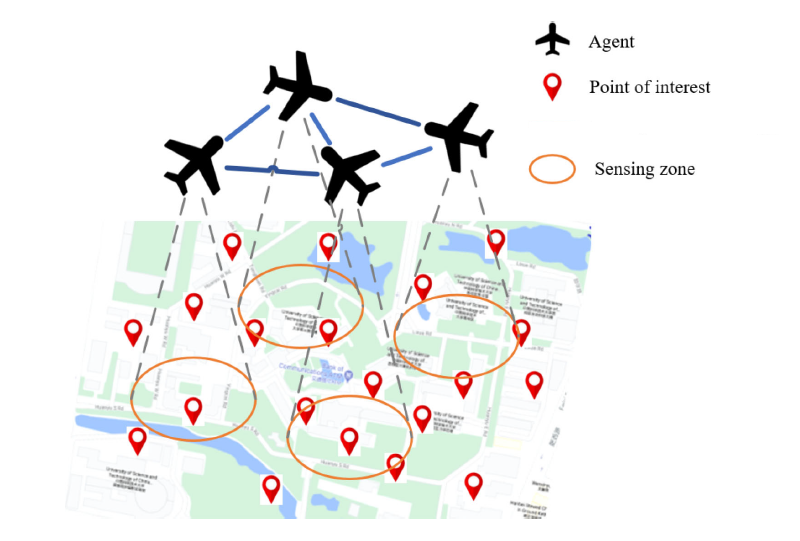
\includegraphics[width=0.9\textwidth]{Images/Scenario.png}
    \centering
    \caption{Possibile scenario di un controllo della copertura dinamico \cite{Articolo_1}.}
    \label{fig: Scenario}
\end{figure}
\vspace{\baselineskip}

Il monitoraggio dinamico di un'area di interesse richiede che, istante per istante, i droni forniscano una visione accurata (o almeno sufficiente) di tutti i target mobili presenti. L'obiettivo generale può variare, come ad esempio l'evitare collisioni tra le imbarcazioni.

Per raggiungere questo obiettivo, è fondamentale garantire una \textit{copertura sufficiente} dell'area. Nel contesto di questo esperimento, le traiettorie dei target saranno predefinite e verranno assegnate posizioni iniziali ai droni. \textbf{Il compito consiste dunque nello scrivere un algoritmo di copertura per determinare le traiettorie dei droni in modo tale che, al termine delle traiettorie dei target, venga raggiunto un grado sufficiente di copertura dell'area.} (vedi \ref{section: algoritmi}).

I droni dovranno quindi "seguire" i target, assicurando una buona visione dell'area di interesse per tutta la durata dell'esperimento. La definizione dettagliata del \textit{grado di copertura sufficiente} verrà fornita nella sezione \ref{section: soluzioniProposte} della tesi.


%\clearpage

\subsection{Formulazione matematica del problema}\label{section: formulMate}

Consideriamo $M$ punti di interesse (\textit{\textbf{Targets dinamici}}) distribuiti in uno spazio di lavoro bidimensionale $W$. Le posizioni dei targets sono denotate da $q_j(t) \in \mathbb{R}^2$, con $j \in \{1, \ldots, M\}$. Un gruppo di $N$ \textit{\textbf{Agenti mobili, dinamici}} (\textit{Agents}), ad un'altezza fissata, è incaricato di monitorare continuamente questi targets. Le posizioni degli agenti sono denotate da $p_i(t) \in \mathbb{R}^2$, con $i \in \{1, \ldots, N\}$.
\\
Si presume che ogni agente abbia una zona di rilevamento limitata, modellata da un'area discoidale con un certo \textit{raggio di copertura} $r \in \mathbb{R}^+$ centrata su se stesso.
\\
Poiché la qualità del rilevamento generalmente degrada con la distanza dal target, il rilevamento basato sulla distanza dell'agente $i$ sul target $j$ è caratterizzato da una \textit{\textbf{funzione di misurazione}}:

\begin{equation}
E_{ij}(p_i(t), q_j(t)) =
\begin{cases} 
    M_P \left( \frac{(l_{ij}(t) - r)^2}{r^4} \right), & \text{se } l_{ij}(t) \leq r^2, \\
    0, & \text{se } l_{ij}(t) > r^2,
\end{cases}
\end{equation}

dove $l_{ij}(t) = \| p_i(t) - q_j(t) \|^2$ è la distanza, all'istante \textit{t}, tra il drone \textit{i} e il target \textit{j}, e $M_P \in \mathbb{R}^+$ è una qualità di rilevamento di picco.  Il modello di rilevamento indica che la qualità del rilevamento del target $j$ raggiunge il picco quando l'agente $i$ coincide con esso, e diminuisce monotonamente quando l'agente $i$ si allontana da esso \cite{Articolo_1}.

\begin{figure}[H]
    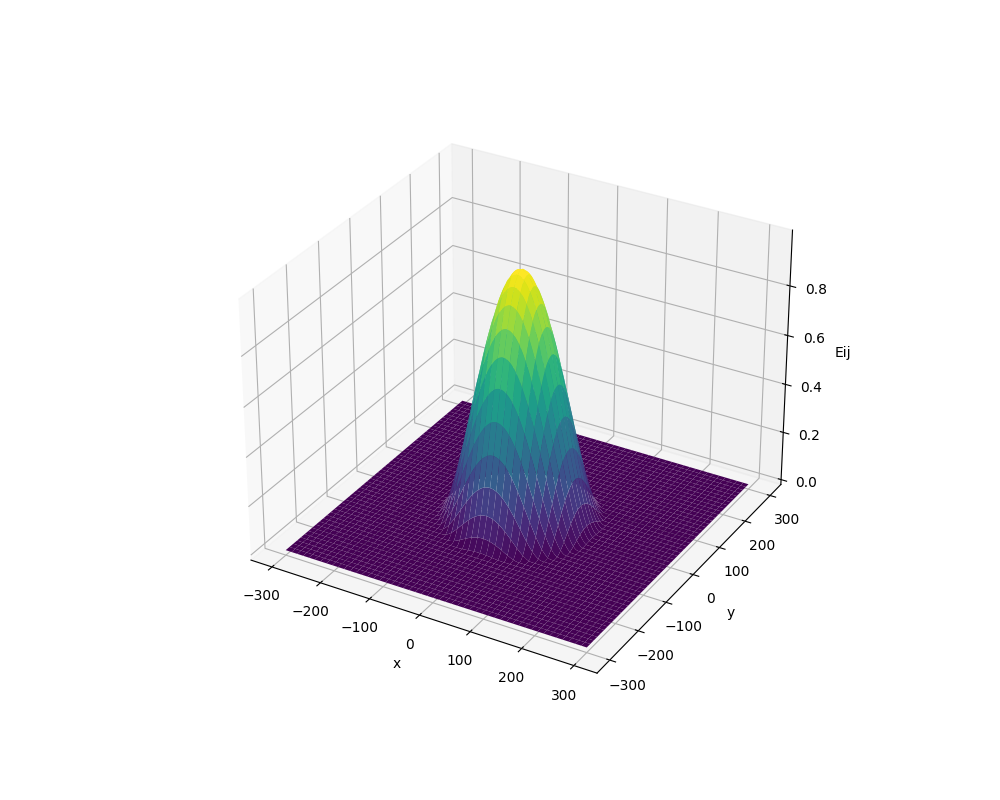
\includegraphics[width=0.8\textwidth]{Images/grafico_Eij.png}
    \centering
    \caption{Funzione di misurazione, mp=1, r=150.}
    \label{fig: funzMisurazione}
\end{figure}
\vspace{\baselineskip}

\newpage

\subsection{Soluzioni proposte}\label{section: soluzioniProposte}

In questa sottosezione viene definita la procedura matematica che stabilisce il \textit{grado di copertura sufficiente}, menzionato nel paragrafo \ref{section: descProblema}. 

\vspace{\baselineskip}

Il controllo della copertura efficace basato su un algoritmo di ascesa del gradiente, con strategia greedy, in questo lavoro ha l'obiettivo di guidare gli agenti mobili affinché garantiscano che ogni target nella regione di interesse sia coperto cumulativamente a un livello desiderato nel tempo \cite{Articolo_1}. Per ogni target $j$, viene definito un \textit{\textbf{indice di copertura $E_j(t)$}}, che quantifica la qualità della copertura al tempo $t$ fornita dai vari agenti. Ogni agente contribuisce all'indice di copertura in base alla propria vicinanza al target, secondo la seguente funzione di misurazione:

\begin{equation}
E_j(t) = \sum_{i=1}^{N} E_{ij} \left( p_i(t), q_j(t) \right), \quad j \text{ fisso}
\label{eq: indiciCopertura}
\end{equation}

Come indicato nella sezione \ref{section: formulMate}, la funzione di misurazione \ensuremath{E_{ij}(p_i(t), q_j(t))} varia nell'intervallo \([0, M_P]\). Di conseguenza, l'indice di copertura \ensuremath{E_j(t)} apparterrà all'intervallo \([0, M_P \cdot N]\).

\vspace{\baselineskip}

Successivamente, viene definito un \textit{\textbf{indice di copertura totale $E(t)$}}, espresso come:


\begin{equation}
E(t) = \sum_{j=1}^{M} \sigma(E_j(t))
\end{equation}

dove:

\begin{equation}
\sigma(E_j(t)) = \frac{\tanh(E_j(t) - E^*) + 1}{2}
\end{equation}


\begin{figure}[H]
    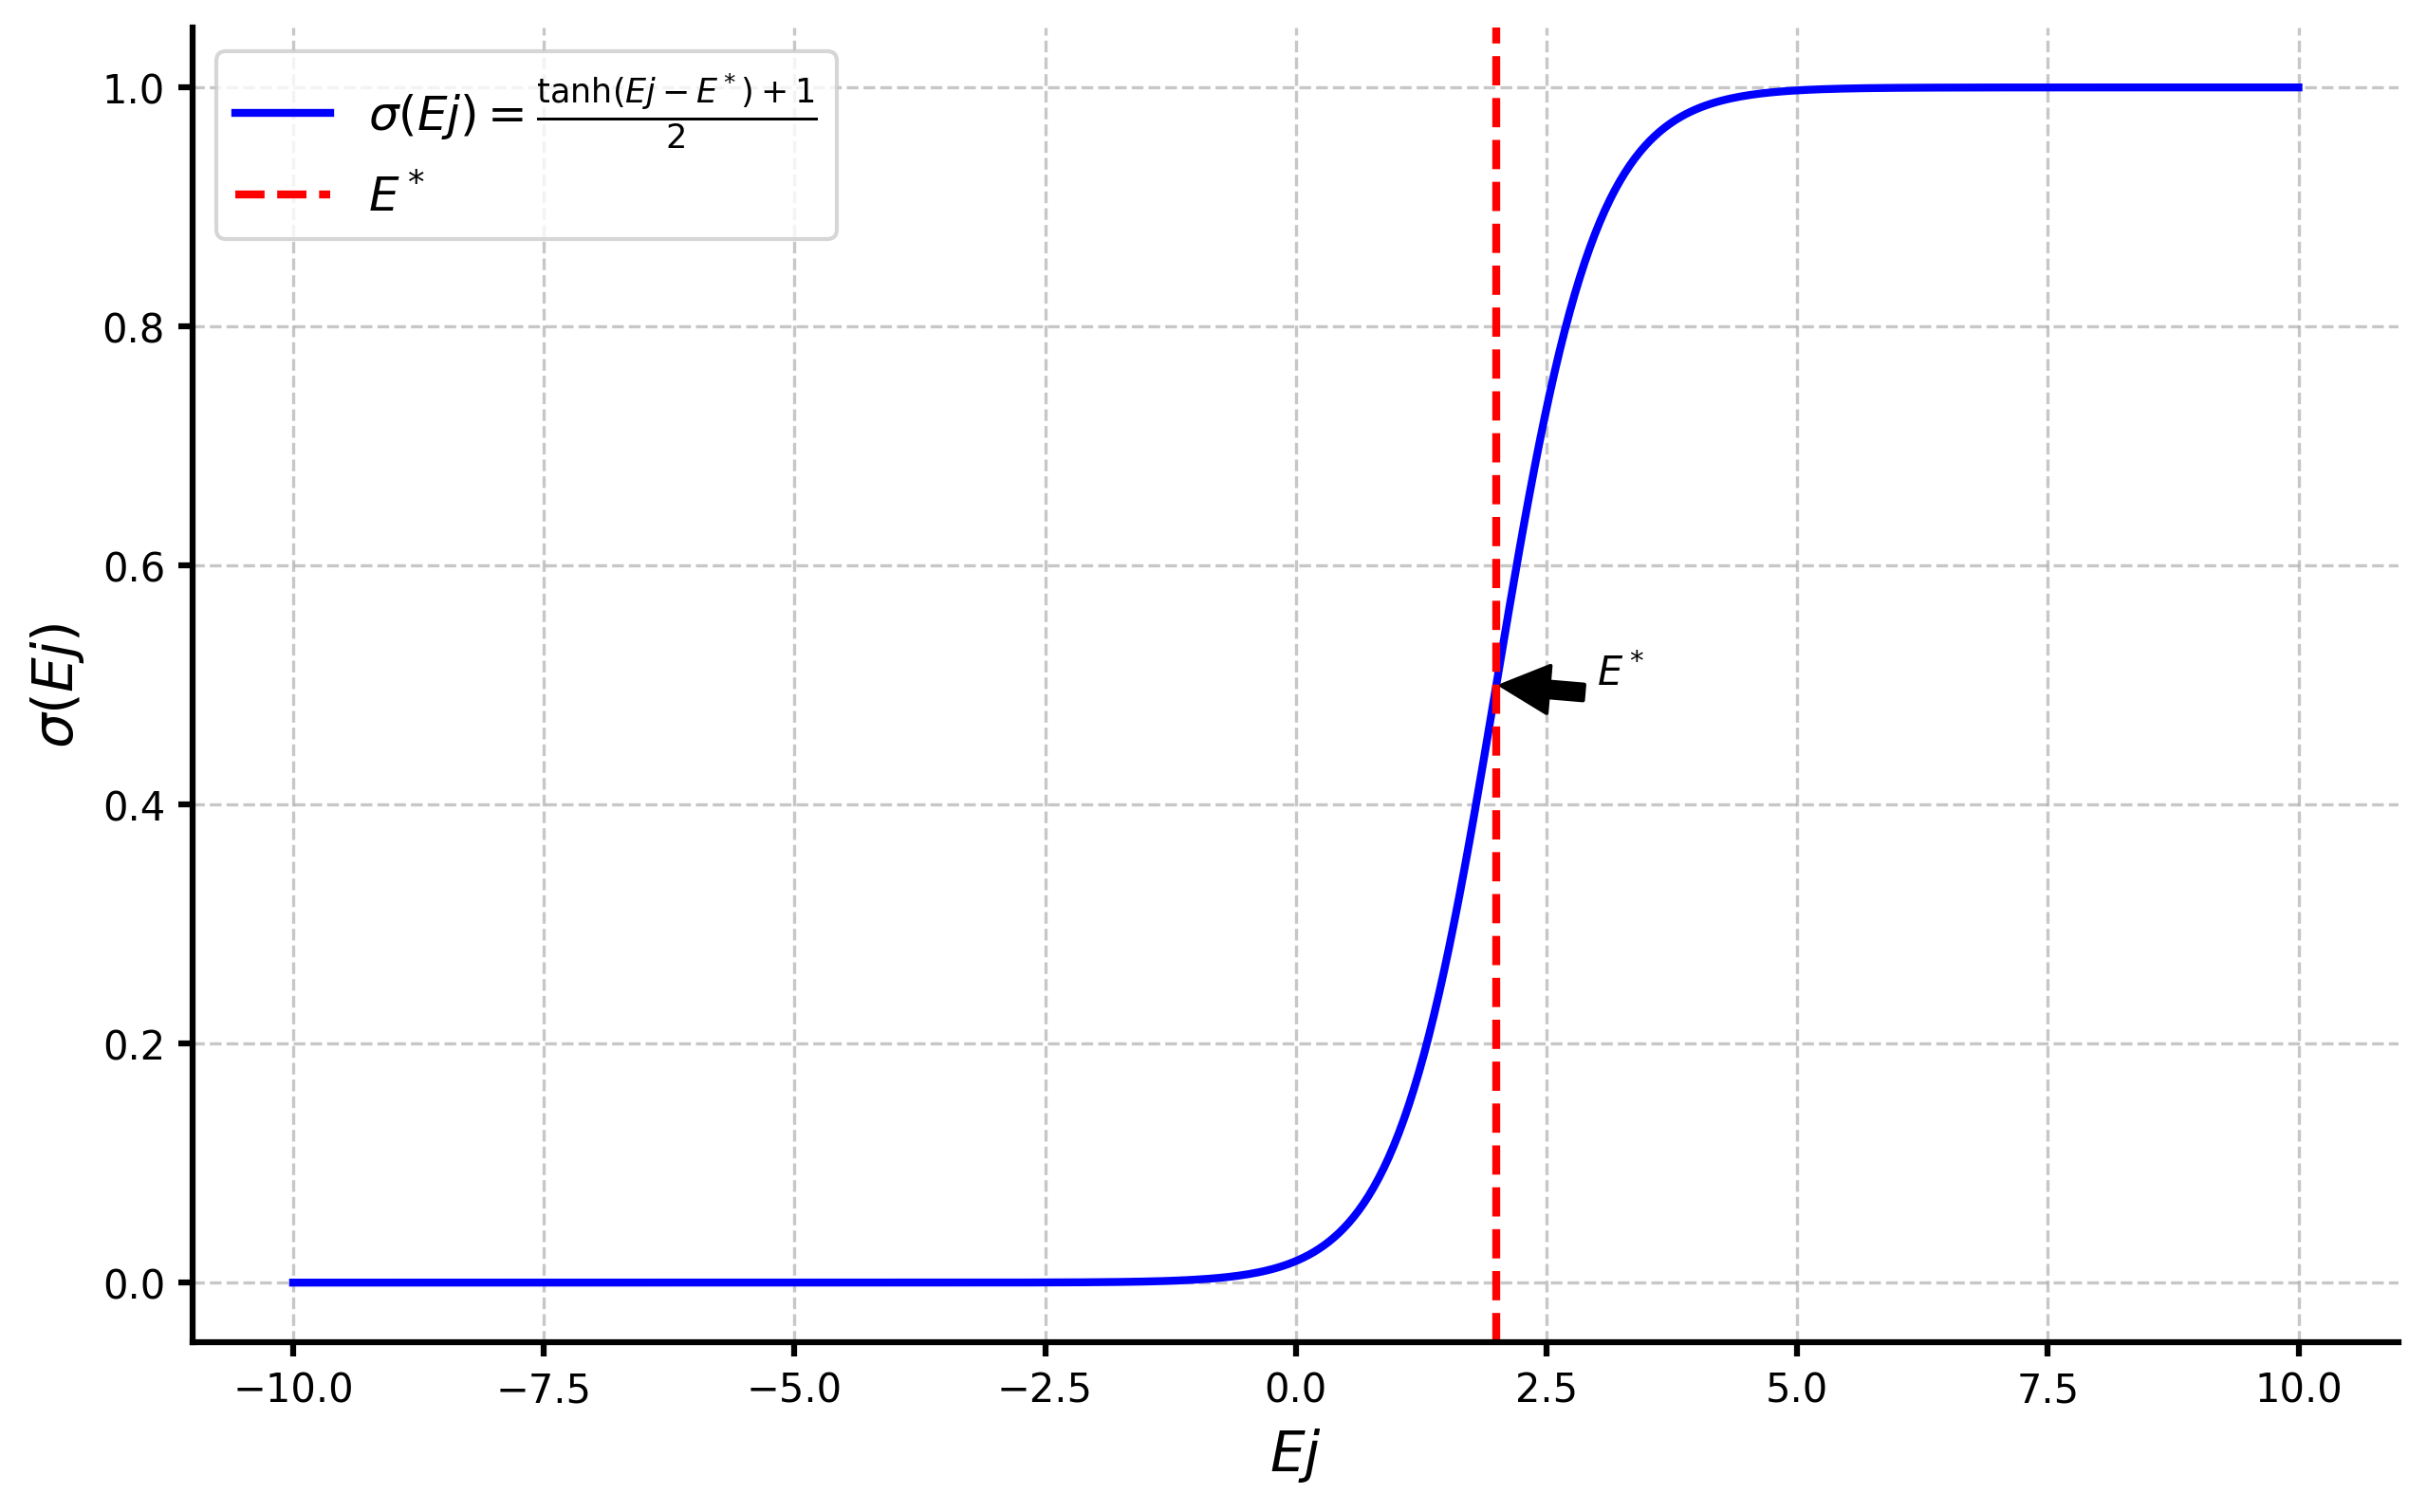
\includegraphics[width=0.7\textwidth]{Images/graficoSig.png}
    \centering
    \caption{Funzione sigmoidale, $E^* = 2$}
    \label{fig: funzSigmoidale}
\end{figure}

La definizione di queste funzioni e indici di copertura è fondamentale per raggiungere l'obiettivo del problema. La soglia \textit{$E^*$} rappresenta un \textit{lower bound index (LB)}, ovvero ogni indice di copertura di un target generico $j$ al tempo $t$ (\ensuremath{E_j(t)}) deve essere maggiore di questa soglia per considerare "accettabile" la copertura fornita dagli agenti. È importante notare che \textit{\textbf{i parametri sono fortemente interdipendenti}}; infatti, in base a $M_P$, varia l'intervallo in cui è contenuta la funzione di misurazione \ensuremath{E_{ij}(p_i(t), q_j(t))} e, di conseguenza, anche gli indici di copertura (\ensuremath{E_j(t)}). È quindi necessario settare i vari parametri caso per caso. Nella simulazione effettuata (vedi \ref{section: simulazione}), sono stati fissati dei parametri accuratamente selezionati, il cui senso logico è spiegato nella sezione \ref{section: settingParametriIniziali}.


\vspace{\baselineskip}

La funzione sigmoidale è stata definita per tener conto di questo ragionamento sulla soglia. L'indice di copertura totale somma i singoli indici di copertura a cui è applicata la sigmoide, in modo che, durante il calcolo del gradiente (vedi \ref{section: algoritmi}), tutti i contributi degli agenti siano considerati.


\vspace{\baselineskip}

Durante la simulazione, verranno generate delle posizioni iniziali degli agenti tali da avere una copertura leggermente inferiore al sufficiente nella situazione iniziale. L'obiettivo sarà quello di sviluppare un algoritmo di copertura dinamica (che verrà analizzato nella sezione \ref{section: algoritmi}) per creare le traiettorie degli agenti e indicare loro come muoversi, al fine di ottenere un \textit{indice di copertura totale} finale significativamente maggiore rispetto a quello iniziale \ensuremath{E(\text{duration}-1) > E(0)}.\\
E' necessario garantire il più alto livello di copertura per il maggior tempo possibile.

\vspace{\baselineskip}

Può succedere, come verrà analizzato in modo esaustivo nella sezione \ref{section: simulazione}, che alcuni indici di copertura singoli al tempo finale \ensuremath{E_{ij}(\text{duration}-1)} siano azzerati o prossimi allo zero.
Questo comportamento non rappresenta un problema, ma è una conseguenza naturale dell'algoritmo di ascesa del gradiente descritto nella sezione \ref{section: analisiRisultati}. L'algoritmo mira a mantenere il grado di copertura più elevato possibile, massimizzando l'indice di copertura totale. Dato che il numero di agenti è inferiore alla metà del numero dei target, è normale che alcuni target possano non essere coperti nell'istante finale. Tuttavia, ciò consente di coprire molti altri target in modo ottimale, contribuendo così all'aumento dell'indice totale.


\newpage


% ALGORITMI--------------------------------------------------------

\section{Algoritmi}\label{section: algoritmi}

\vspace{\baselineskip}

Come anticipato nell'introduzione, l'obiettivo di questo progetto è sviluppare un algoritmo di copertura dinamico (\textbf{dynamic coverage algorithm}) per determinare le traiettorie degli agenti, al fine di massimizzare l'indice di copertura totale \ensuremath{E}.

\vspace{\baselineskip}

Gli algoritmi proposti si basano tutti sul \textbf{metodo di ascesa del gradiente} come fondamento implementativo. Un algoritmo basato sull'ascesa del gradiente è una tecnica di ottimizzazione iterativa utilizzata per individuare il massimo di una funzione obiettivo. L'idea principale consiste nell'aggiornare iterativamente le variabili nella direzione del gradiente della funzione obiettivo rispetto a queste variabili, al fine di aumentare il valore della funzione \cite{LibroAscesaGradiente}.

\vspace{\baselineskip}

Nelle sezioni seguenti verranno illustrati tre differenti tipi di algoritmi di copertura dinamica basati sull'ascesa del gradiente. Le versioni seconda e terza saranno estese per risolvere problemi di collisione tra gli agenti nell'istante finale.

\begin{figure}[H]
    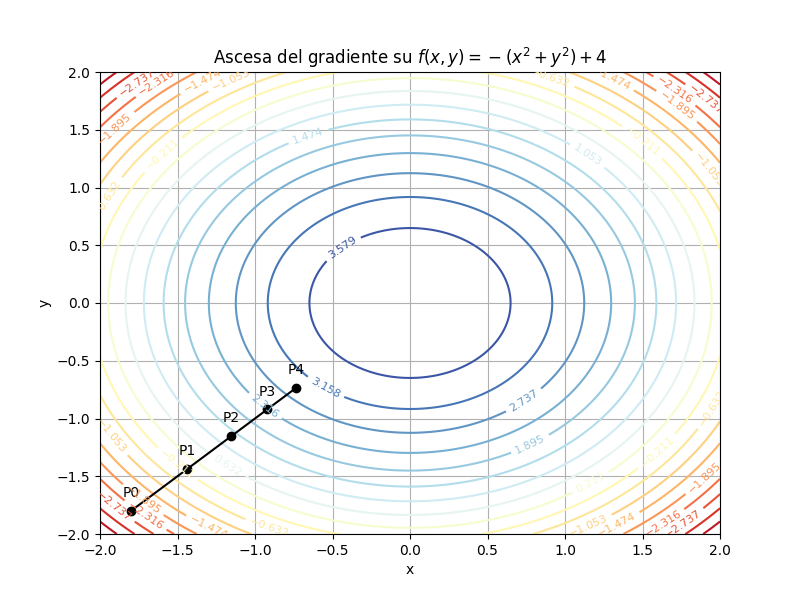
\includegraphics[width=1\textwidth]{Images/gradient_ascent_example.png}
    \centering
    \caption{Ascesa del gradiente}
    \label{fig: ascesaGradiente}
\end{figure}

\newpage

\subsection{Algoritmo di coverage V1: algoritmo di ascesa del gradiente classico}\label{section: v1}

Nell'ambito del presente progetto di controllo della copertura dinamica, l'algoritmo di ascesa del gradiente viene impiegato per aggiornare le posizioni degli agenti mobili, come droni, determinando le loro traiettorie in modo da massimizzare una funzione obiettivo che rappresenta la copertura totale dell'area di interesse, ovvero l'indice di copertura totale \ensuremath{E(t)}.\
Gli agenti calcolano il gradiente della funzione di copertura rispetto alle loro posizioni e a quelle dei target al tempo corrente. Successivamente, aggiornano le loro traiettorie seguendo la direzione del gradiente, migliorando iterativamente la copertura complessiva dell'area.

\vspace{\baselineskip}

\begin{algorithm}[H]
\SetAlgoLined
\KwResult{Massimizzare la copertura totale $E$}
\For{ogni $t$}{
  \For{ogni agente $i$}{
    Decidere la direzione in cui muovere l'agente per massimizzare la copertura\;
    \[
    \mu_i = \left. \frac{\partial E}{\partial p_i} \right|_{p_i = p_i(t), q_i = q_i(t)} (p_1, \ldots, p_N, q_1, \ldots, q_N)
    \]
    L'agente si muove con passo di salita $\epsilon$\;
    \textcolor{red}{\textbf{$p_i(t+1) = p_i(t) + \epsilon \mu_i(t)$}}\;
  }
}
\caption{V1: Algoritmo di coverage dinamico con ascesa del gradiente}
\end{algorithm}

\vspace{\baselineskip}

In questo contesto, $\epsilon$\ rappresenta il passo di salita. Questo parametro è cruciale per l'aggiornamento delle posizioni degli agenti mobili ed è direttamente responsabile della velocità con cui gli agenti si muovono lungo la traiettoria determinata dal gradiente della funzione obiettivo.

\vspace{\baselineskip}
Come descritto in dettaglio nella sezione \ref{section: descProblema}, è possibile che al termine dell'esecuzione dell'algoritmo alcuni indici di copertura individuali \ensuremath{E_{ij}(\text{duration}-1)} risultino pari a zero o prossimi allo zero. Questo fenomeno non rappresenta un'anomalia, ma un comportamento previsto dell'algoritmo di ascesa del gradiente, il cui obiettivo principale è la massimizzazione dell'indice di copertura totale. Di conseguenza, alcuni target potrebbero non essere coperti al termine della simulazione.\\

\textit{\textbf{Un problema emergente}} in questa situazione è che gli agenti, per massimizzare la copertura, possono convergere verso posizioni finali molto vicine tra loro al tempo \( t = \text{duration} \), aumentando il rischio di \textit{\textbf{collisione}}. Questo è un problema ben noto nel contesto del coverage dinamico, dove la priorità alla copertura totale può portare a densità elevate di agenti in aree specifiche.\\

Per mitigare il rischio di collisione e migliorare la distribuzione spaziale degli agenti, sono state sviluppate due ulteriori versioni dell'algoritmo. Queste versioni estendono la versione base dell'algoritmo di ascesa del gradiente, introducendo meccanismi che favoriscono una separazione adeguata tra gli agenti, garantendo una copertura efficace senza incorrere in collisioni esagerate.\\

Nel contesto del controllo di copertura dinamica, il problema della collisione tra agenti è un aspetto cruciale da gestire. Quando più agenti, come droni, operano nello stesso spazio per monitorare una serie di punti di interesse, c'è un rischio significativo che le loro traiettorie si intersechino, portando a collisioni. Questo è particolarmente problematico alla fine dell'esecuzione dell'algoritmo di copertura, quando gli agenti tendono a convergere verso le aree con alta densità di target.

Per affrontare questo problema, diverse strategie di controllo dell'evitamento delle collisioni (\textit{collision avoidance}) sono state proposte in letteratura. Alcuni approcci utilizzano tecniche di ottimizzazione che includono vincoli di distanza minima tra gli agenti, mentre altri implementano algoritmi di controllo distribuito che permettono agli agenti di coordinarsi per evitare le collisioni in tempo reale. Un esempio di queste tecniche è l'uso di funzioni potenziali che generano forze repulsive tra gli agenti quando si avvicinano troppo l'uno all'altro \cite{collisionAvoidance} (come fatto in V3: sezione \ref{section: v3}). 



\subsection{Algoritmo V2: aggiunta di un moto Browniano}\label{section: v2}

In questa seconda versione dell'algoritmo, le posizioni degli agenti vengono aggiornate non solo utilizzando il gradiente della funzione obiettivo, ma anche includendo una componente stocastica derivante dal \textbf{moto browniano}. Questo approccio introduce una variazione casuale nelle traiettorie degli agenti, migliorando la loro capacità di esplorazione e riducendo il rischio di convergenza in posizioni subottimali.

\vspace{\baselineskip}
\begin{algorithm}[H]
\SetAlgoLined
\KwResult{Massimizzare la copertura totale $E$}
\For{ogni $t$}{
    \textcolor{red}{Calcolo della componente Browniana $\eta_i(t)$}\\
  \For{ogni agente $i$}{
    Decidere la direzione in cui muovere l'agente per massimizzare la copertura\;
    \[
    \mu_i = \left. \frac{\partial E}{\partial p_i} \right|_{p_i = p_i(t), q_i = q_i(t)} (p_1, \ldots, p_N, q_1, \ldots, q_N)
    \]
    L'agente si muove con passo di salita $\epsilon$\;
    \textcolor{red}{\textbf{$p_i(t+1) = p_i(t) + \epsilon \mu_i(t)$ + $\eta_i(t)$}}\;
  }
}
\caption{V2: Algoritmo di coverage dinamico, aggiunta moto di Browniano}
\end{algorithm}
\vspace{\baselineskip}

Il moto browniano, noto anche come movimento aleatorio, è un modello matematico utilizzato per descrivere il comportamento di particelle che si muovono in modo casuale in un fluido. Questo fenomeno prende il nome dal botanico Robert Brown, che per primo osservò il movimento irregolare di particelle microscopiche in sospensione nel 1827. Il moto browniano è caratterizzato da una traiettoria irregolare e imprevedibile, dove ogni passo successivo è indipendente dal precedente e segue una distribuzione di probabilità specifica \cite{StochasticProcesses}.\\

Il moto browniano può essere modellato matematicamente come un processo stocastico, spesso descritto da equazioni differenziali stocastiche. In particolare, il modello di Wiener è comunemente utilizzato per rappresentare il moto browniano. Questo modello considera la traiettoria di una particella come una somma di incrementi casuali, ciascuno distribuito normalmente con media zero e varianza proporzionale al tempo. La funzione di densità di probabilità per la posizione della particella a un tempo futuro è quindi una distribuzione gaussiana, il cui centro si sposta con il tempo e la cui larghezza aumenta proporzionalmente alla radice quadrata del tempo \cite{StochasticProcesses}.\\

Nel contesto degli algoritmi di ottimizzazione e controllo, il moto browniano può essere utilizzato per introdurre una componente stocastica nei movimenti degli agenti. Questa componente stocastica permette una migliore esplorazione dello spazio delle soluzioni, contribuendo a evitare il problema della convergenza a soluzioni subottimali. In particolare, l'introduzione di una variazione casuale nei movimenti degli agenti consente loro di esplorare aree più ampie dello spazio di ricerca, aumentando così la probabilità di trovare soluzioni globali ottimali. Ad esempio, l'algoritmo di ottimizzazione basato sul moto browniano dei gas (GBMO) combina i principi fisici del moto browniano con strategie di ottimizzazione per migliorare la ricerca di soluzioni ottimali in spazi complessi \cite{Abdechiri2013}. Altri studi dimostrano che il moto browniano può essere combinato con altri algoritmi di ottimizzazione, come l'algoritmo del volo della farfalla e l'ottimizzazione degli stormi di particelle, per migliorare ulteriormente le prestazioni e la convergenza \cite{Sowjanya2021}, \cite{Xiaohong2012}.

\vspace{\baselineskip}

\textit{\textbf{La componente browniana}} \(\eta_i(t)\) è definita come:

\begin{equation}
\eta_i(t) = \begin{bmatrix}
\text{gauss}_i(t) \cdot \cos(\theta_i(t)) \\
\text{gauss}_i(t) \cdot \sin(\theta_i(t))
\end{bmatrix}
\end{equation}

dove:

\begin{equation}
\theta_i(t) \sim \mathcal{U}(0, 2\pi)
\end{equation}
rappresenta la \textit{\textbf{direzione casuale}}, distribuita uniformemente nell'intervallo \([0, 2\pi]\).

\begin{equation}
\text{gauss}_i(t) \sim \mathcal{N}(\mu, \sigma^2)
\end{equation}

rappresenta \textit{\textbf{l'intensità del moto}} browniano, distribuita secondo una distribuzione gaussiana con media \(\mu\) e varianza \(\sigma^2\).\\

Questa componente aggiuntiva introduce una variazione casuale nel movimento degli agenti, permettendo una migliore esplorazione dello spazio e contribuendo a evitare che gli agenti si raggruppino in posizioni subottimali.

\begin{figure}[H]
    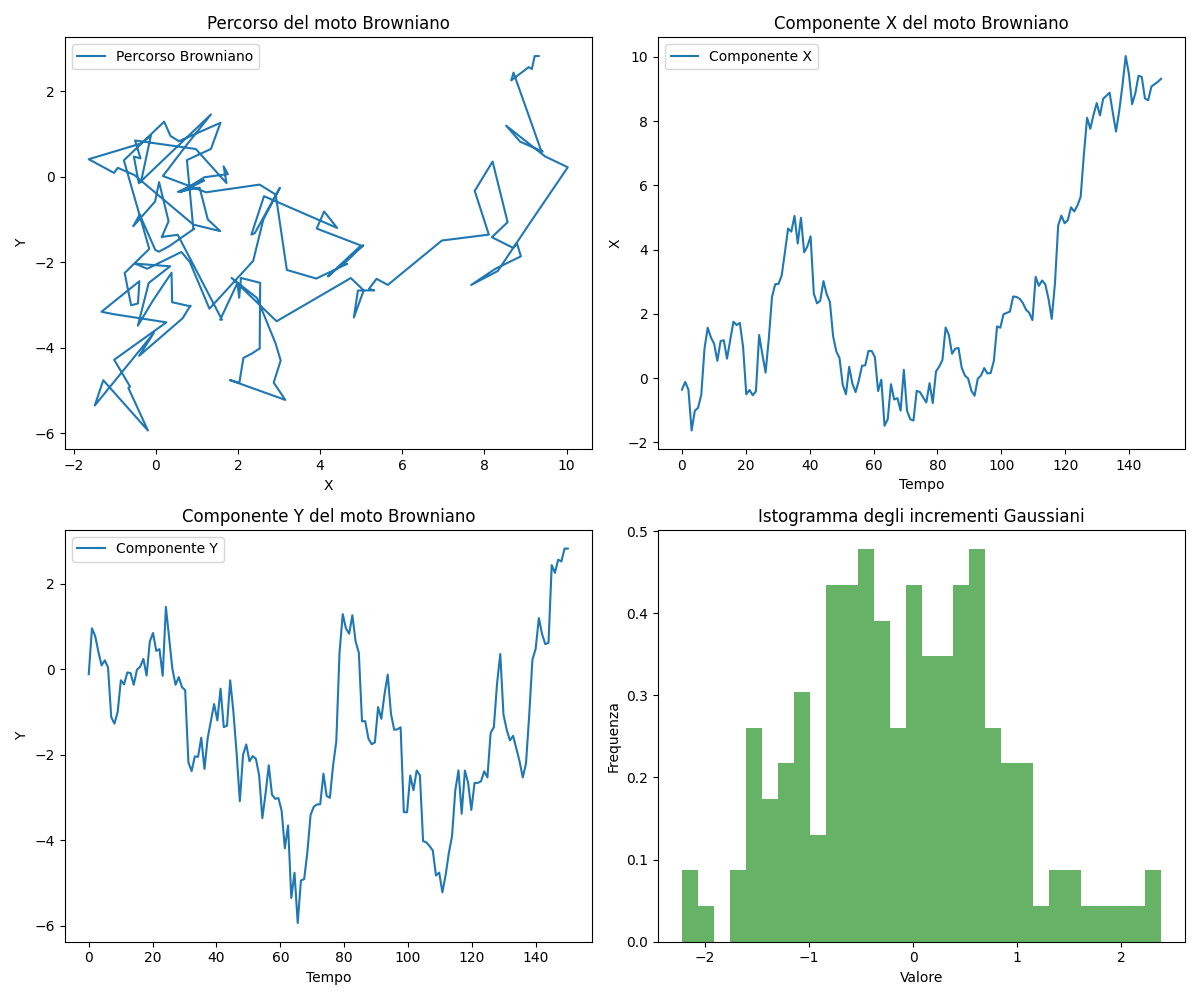
\includegraphics[width=1\textwidth]{Images/Brownian_motion_components.png}
    \centering
    \caption{Grafici del moto Browniano}
    \label{fig: motoBrowniano}
\end{figure}

La Figura \ref{fig: motoBrowniano} illustra diverse caratteristiche del moto browniano. Il grafico in alto a sinistra mostra la traiettoria in due dimensioni di una particella che segue un moto browniano, evidenziando la natura casuale e imprevedibile del percorso. I grafici in alto a destra e in basso a sinistra mostrano rispettivamente le componenti X e Y del moto browniano nel tempo, che evidenziano come queste componenti variano casualmente. Infine, l'istogramma in basso a destra rappresenta la distribuzione degli incrementi gaussiani, confermando che questi incrementi seguono una distribuzione normale con media zero.

\newpage

\subsection{Algoritmo V3: aggiunta di un potenziale repulsivo}\label{section: v3}

In questa terza versione dell'algoritmo, le posizioni degli agenti vengono aggiornate non solo utilizzando il gradiente della funzione obiettivo, ma anche includendo una componente di \textbf{potenziale repulsivo}. Questo approccio introduce una forza repulsiva tra gli agenti quando la distanza tra di loro è inferiore a una certa soglia \(\delta\). L'obiettivo principale di questa componente è evitare collisioni tra gli agenti durante la loro operatività, migliorando la sicurezza e l'efficacia del controllo della copertura.

\vspace{\baselineskip}
\begin{algorithm}[H]
\SetAlgoLined
\KwResult{Massimizzare la copertura totale $E$}
\For{ogni $t$}{
  \For{ogni agente $i$}{
    \textcolor{red}{Calcolo del potenziale repulsivo}\\
    Decidere la direzione in cui muovere l'agente per massimizzare la copertura\;
    \[
    \mu_i = \left. \frac{\partial E}{\partial p_i} \right|_{p_i = p_i(t), q_i = q_i(t)} (p_1, \ldots, p_N, q_1, \ldots, q_N)
    \]
    L'agente si muove con passo di salita $\epsilon$\;
    \textcolor{red}{\textbf{$p_i(t+1) = p_i(t) + \epsilon \mu_i(t)$ + $\eta$}}\;
  }
}
\caption{V3: Algoritmo di coverage dinamico, aggiunta di un potenziale repulsivo}
\end{algorithm}

\vspace{\baselineskip}

La \textbf{forza repusliva totale \(\eta\)} è la somma delle componenti repulsive calcolate per tutti gli agenti \(k\) diversi da \(i\):

\begin{equation}
\eta = \sum_{k \ne i} \eta^k_i(t)
\end{equation}

dove la componente repulsiva \(\eta^k_i(t)\) è calcolata come segue:

\begin{equation}
\eta^k_i(t) = 
\begin{cases} 
\left[ \textcolor{blue}{\frac{p_i(t) - p_k(t)}{d_{ik}(t)}} \right] \cdot \left[ \textcolor{orange}{\frac{\delta - d_{ik}(t)}{d_{ik}(t)}} \right] & \text{se } d_{ik}(t) \leq \delta \\
0 & \text{se } d_{ik}(t) > \delta 
\end{cases}
\label{eq:potenziale_repulsivo}
\end{equation}

dove \(d_{ik}(t) = \| p_i(t) - p_k(t) \|\) rappresenta la distanza tra l'agente \(i\) e l'agente \(k\) al tempo \(t\).\\

Se la distanza è inferiore alla soglia \(\delta\), viene calcolata una forza repulsiva. Il primo termine \textcolor{blue}{in blu} è il versore che indica \textit{la direzione di allontanamento} dall'agente \(k\). Il secondo termine \textcolor{orange}{in arancione} rappresenta \textit{l'intensità della forza repulsiva}, che aumenta inversamente proporzionale alla distanza tra gli agenti: più \(i\) e \(k\) sono vicini, maggiore è la forza repulsiva.\\
\textit{Questo fattore è critico per garantire che la forza repulsiva sia efficace solo quando necessario, senza interferire con il compito principale di massimizzare la copertura.}

\vspace{\baselineskip}

Viene riportato il grafico dell' \textcolor{orange}{intensità della forza repulsiva} che mostra come l'intensità della forza repulsiva decresca all'aumentare della distanza tra gli agenti \(i\) e \(k\). Quando la distanza è inferiore a una certa soglia \(\delta\), la forza repulsiva è alta, mentre diminuisce rapidamente man mano che la distanza aumenta, tendendo a zero quando la distanza è maggiore di \(\delta\).

\begin{figure}[H]
    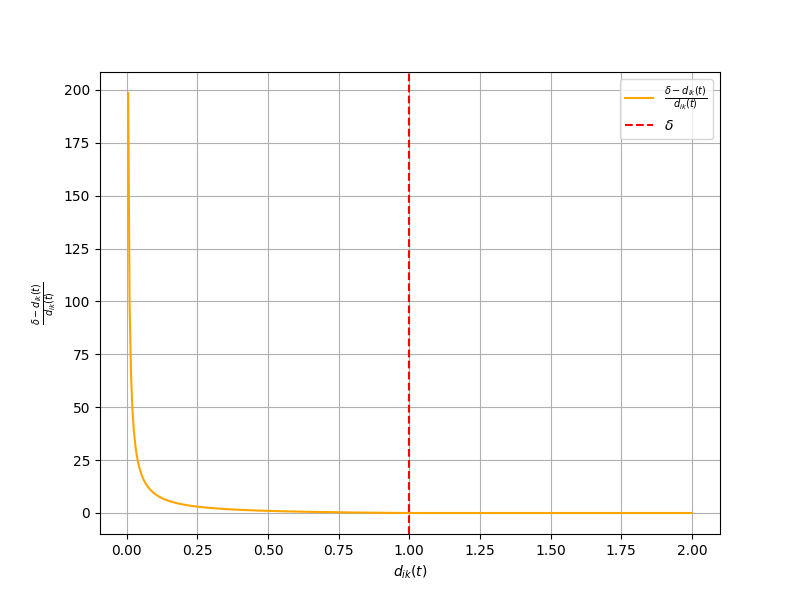
\includegraphics[width=1\textwidth]{Images/intensPotRep.png}
    \centering
    \caption{Intensità del potenziale repulsivo}
    \label{fig: intensPotRep}
\end{figure}

\vspace{\baselineskip}


Il potenziale repulsivo è una tecnica ampiamente utilizzata nel campo della robotica e del controllo multi-agente per prevenire le collisioni. La forza repulsiva cresce man mano che gli agenti si avvicinano tra loro, inducendo un movimento che li spinge a distanziarsi. Questo metodo garantisce che gli agenti mantengano una distanza di sicurezza reciproca, riducendo il rischio di collisioni durante il movimento.\\
Secondo Hao et al., il potenziale repulsivo è fondamentale per il controllo di formazione e la manutenzione della connettività nei sistemi multi-agente. La forza repulsiva viene calcolata in base alla distanza tra gli agenti, aumentando esponenzialmente quando la distanza scende sotto una soglia di sicurezza, generando un'azione di repulsione che allontana gli agenti l'uno dall'altro \cite{MDPI_Hao}. Questo meccanismo è particolarmente utile nel contesto del coverage dinamico, dove gli agenti devono cooperare per coprire un'area di interesse senza collidere tra loro.\\
In un altro studio, Jiang et al. descrivono come l'utilizzo di potenziali repulsivi possa migliorare l'efficacia della copertura dinamica, specialmente in scenari complessi con molti agenti che operano in prossimità. I potenziali repulsivi permettono agli agenti di distribuire uniformemente lo spazio di copertura, ottimizzando l'efficienza e riducendo i rischi di collisione \cite{MDPI_Jiang}.\\
Inoltre, Nagy et al. hanno condotto uno studio sul comportamento dei sistemi multi-agente mobili durante la costruzione di campi di potenziale, dimostrando che le forze repulsive aiutano a mantenere gli agenti separati e ad evitare collisioni \cite{Nagy2009}. L'integrazione del controllo reattivo e telerobotico nei sistemi robotici multi-agente è stata esplorata da Arkin e Ali, evidenziando come le forze repulsive tra robot permettono una convergenza sicura e coordinata \cite{Arkin1994}. Infine, Mabrouk e McInnes hanno introdotto un modello per simulare il comportamento emergente dei robot a sciame, utilizzando campi di potenziale basati su forze attrattive e repulsive \cite{Mabrouk2008}.

\vspace{\baselineskip}

Questo approccio assicura che ogni agente consideri la presenza degli altri agenti nel suo ambiente e regoli il proprio movimento di conseguenza, \textit{\textbf{evitando collisioni}} e mantenendo una copertura efficace dell'area di interesse.

\newpage

% IMPLEMENTAZIONE ALGORITMI----------------------------------------

\section{Implementazione degli algoritmi}\label{section: algoritmiImp}
\vspace{\baselineskip}
L'intero progetto di tesi è stato sviluppato utilizzando il linguaggio di programmazione Python. In questa sezione, verranno illustrati \textsc{solo i punti cruciali della logica del programma}, partendo dalle operazioni preliminari fino ad arrivare alla reale implementazione degli algoritmi di coverage discussi nella sezione \ref{section: algoritmi}.\\
Per l'analisi del codice completo è possibile fare riferimento a (\href{https://github.com/IvanNece/Dynamic_Coverage_Control_Area_Portuale_Tesi_Necerini}{Source code}).\\
Il codice è strutturato come mostrato nelle figure \ref{fig: pathCodice} e \ref{fig: zoomAlgoritmi}.

\begin{figure}[htbp]
    \begin{minipage}[b]{0.5\linewidth}  % Definisci la larghezza del primo minipage al 50% della larghezza della pagina
        \centering
         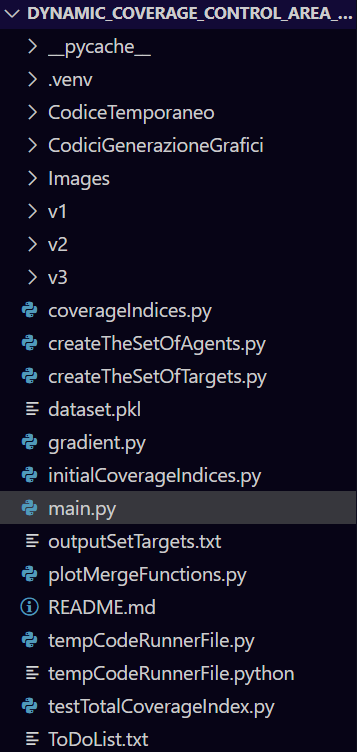
\includegraphics[width=0.8\textwidth, height=0.7\textheight]{Images/pathCodice.png}  % Inserisci la prima immagine
        \caption{Organizzazione del codice}
        \label{fig: pathCodice}
    \end{minipage}
    \hspace{0.5cm}  % Aggiungi uno spazio orizzontale tra le immagini
    \begin{minipage}[b]{0.5\linewidth}  % Definisci la larghezza del secondo minipage al 50% della larghezza della pagina
        \centering
         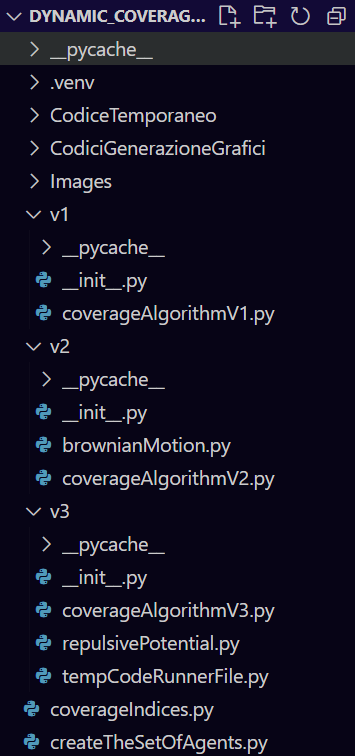
\includegraphics[width=0.8\textwidth, height=0.7\textheight]{Images/zoomAlgoritmi.png}  % Inserisci la seconda immagine
        \caption{Zoom nelle cartelle degli algoritmi}
        \label{fig: zoomAlgoritmi}
    \end{minipage}
\end{figure}


\subsection{Operazioni preliminari}\label{section: operPreliminari}

\textit{\textbf{L'unico dato in input di questo progetto è un dataset}}, salvato in un file \textit{.pickle}. Come illustrato in figura \ref{fig: traiettorieTarget}, il dataset contiene le traiettorie dei target. Una volta caricato, il dataset (50 traiettorie in una regione di 800 x 800) si presenta nella seguente struttura:

\begin{itemize}
    \item \verb|np.shape(dataset[i][0])=(351, 4)|
    \item \verb|np.shape(dataset[i][1])=(351, 2) |
\end{itemize}

dove i è l'indice della traiettoria e 0,1 indica stato vero (0) con 4 componenti (posizione x, posizione y, velocità x, velocità y) e misure (1) con 2 componenti della posizione, in tutto ciò \textit{l'intervallo di campionamento è di 1 secondo}. Quindi il dataset è una lista di tuple, ognuna di esse contiene due array numpy, uno per rappresentare lo stato vero della traiettoria e l'altro per le \textbf{misurazioni} (che rappresentano i dati effettivi delle coordinate della traiettoria considerando lo stato vero + un rumore di misura additivo).

\begin{figure}[H]
    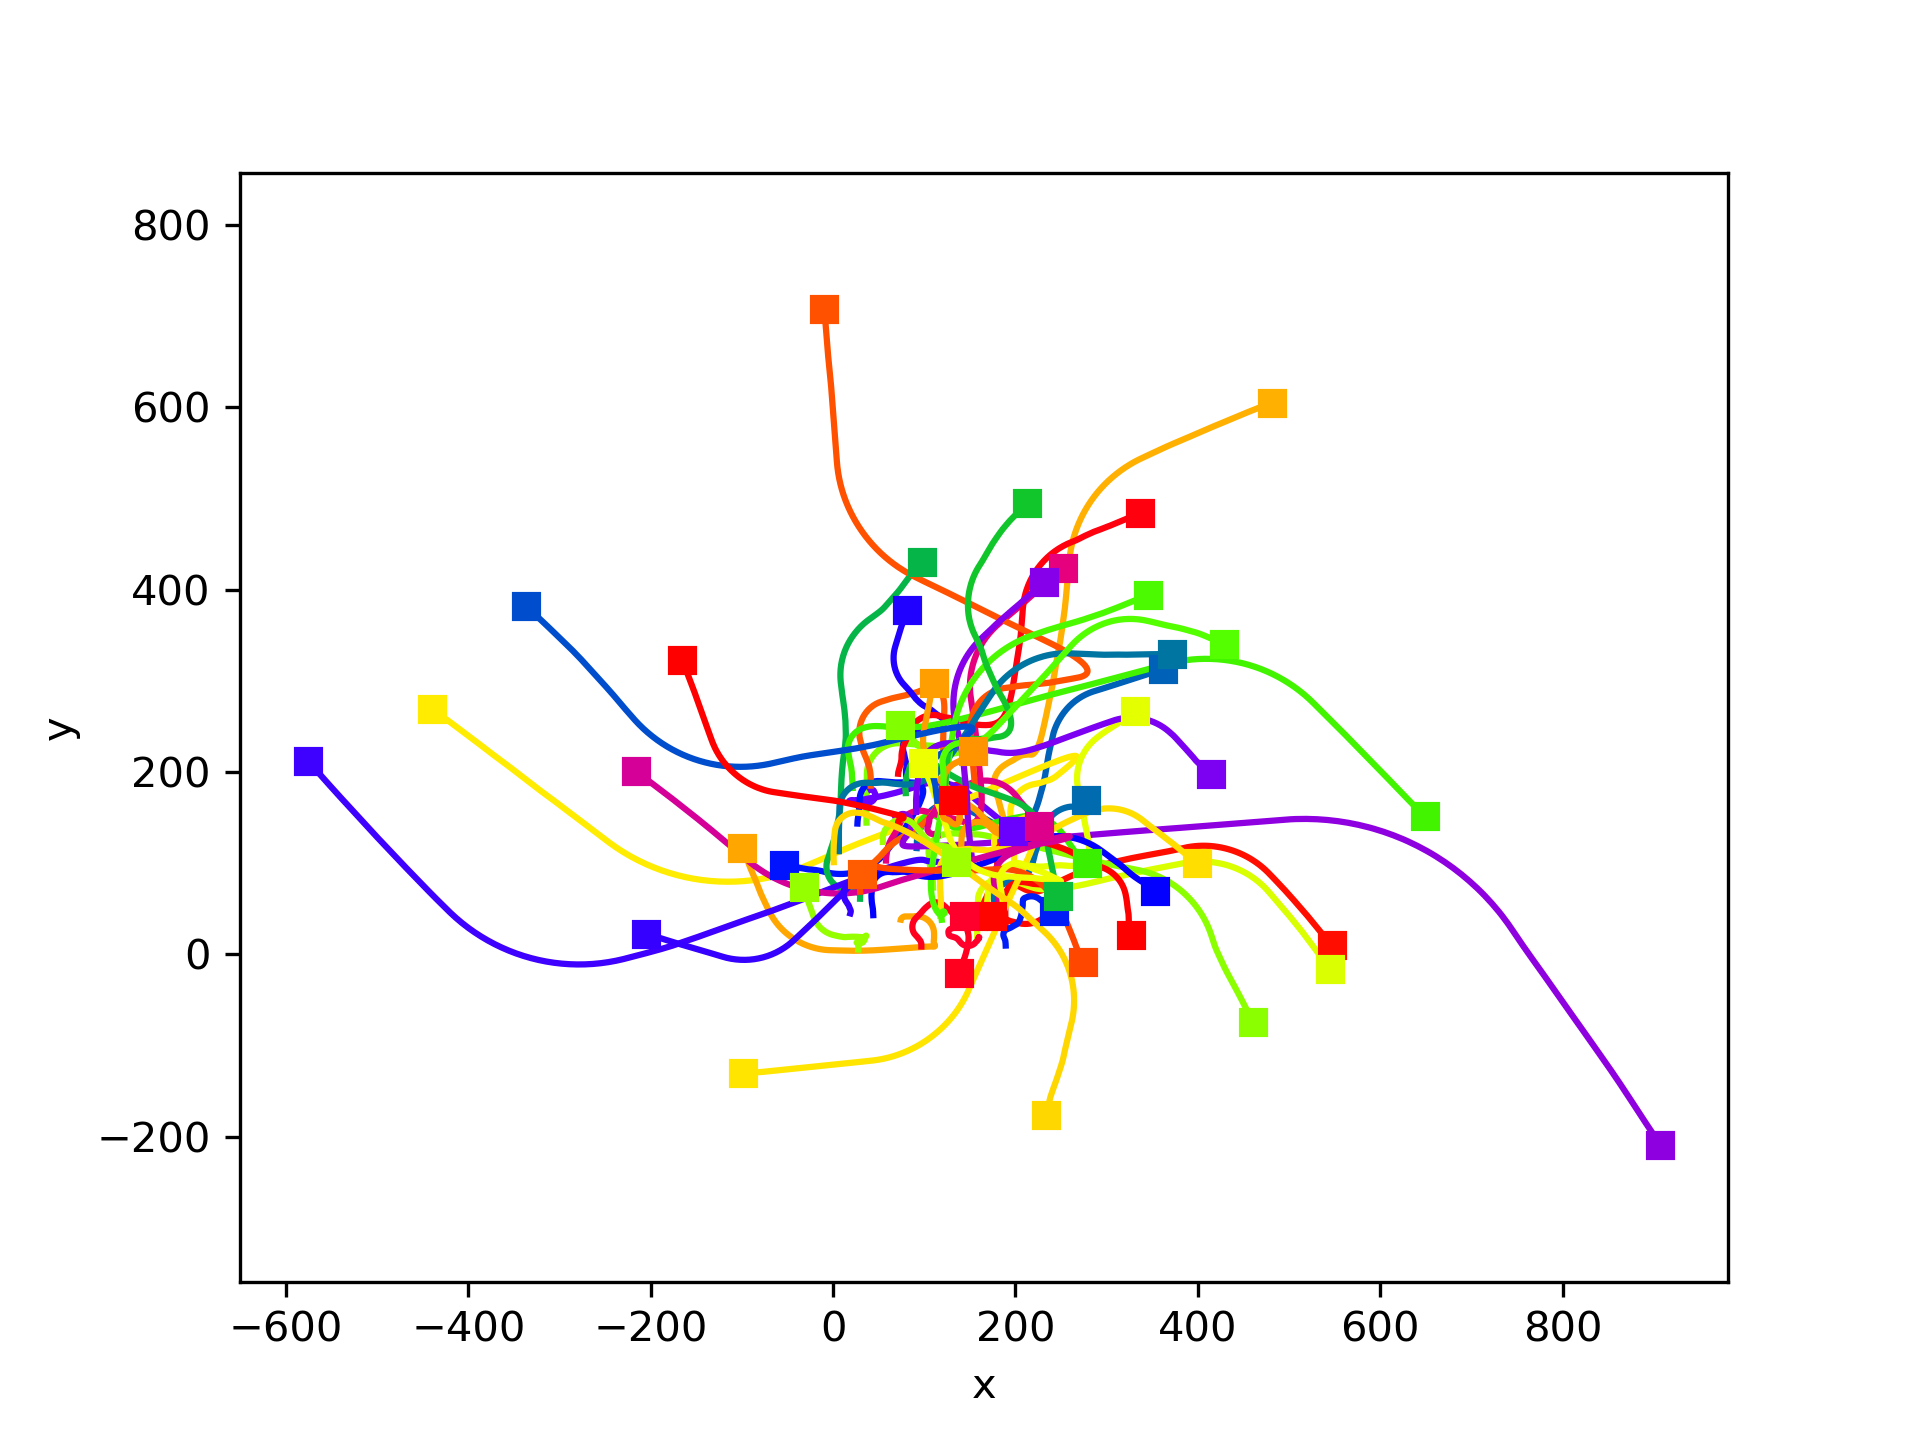
\includegraphics[width=1\textwidth]{Images/datasetTargets.png}
    \centering
    \caption{Dataset traiettorie dei target}
    \label{fig: traiettorieTarget}
\end{figure}

Per simulare il progetto, ad ogni esecuzione del programma vengono selezionate casualmente 10 traiettorie (\textit{numTargets}) della durata di 150 secondi (\textit{duration}). Maggiori dettagli sul settaggio dei parametri sono disponibili nella sezione \ref{section: simulazione}. Di seguito è riportato il cuore della funzione responsabile della creazione del dataset di traiettorie dei target utilizzate. È importante notare che viene estratta solo la parte delle \textbf{misurazioni}, che è quella di nostro interesse. Ovviamente prima di chiamare la funzione, nel main, il dataset è stato estratto dal file pickle (vedi \cite{Pickle}).


\begin{code}{Metodo "buildTheSet()" di \textit{createTheSetOfTargets}}
def buildTheSet(numTrajectories: int, inputDataset: list, duration: int):
    selectedTrajectories = []
    try:
        for _ in range(numTrajectories):
            random_trajectory_index = np.random.choice(len(inputDataset))
            # Ottieni la traiettoria corrispondente all'indice casuale
            random_trajectory = inputDataset[random_trajectory_index]
            # Tronca la traiettoria ai primi "duration" secondi
            truncated_real_state = random_trajectory[0][:duration]
            truncated_measurement = random_trajectory[1][:duration]
            # Aggiungi la traiettoria troncata alla lista delle traiettorie selezionate
            selectedTrajectories.append((truncated_real_state, truncated_measurement))
    except Exception as e:
        print("Errore durante la creazione dello scenario:", e)
    
    return selectedTrajectories
\end{code}

\begin{code}{Estrazione delle misure nel \textit{main}}
# Estrarre solo la parte truncated_measurement
    targets = [truncated_measurement for _, truncated_measurement in createdDatasetOfTargets]
    targetTrajectories = np.array(targets)
\end{code}

La struttura dell'array \textit{targetTrajectories} sarà dunque \textsc{[numTargets]x[duration]x[2]} dove 2 rappresenta le due coordinate x e y.

\vspace{\baselineskip}

Successivamente, è necessario andare a creare delle posizioni iniziali degli agenti, dei quali, per adesso, non è presente nessuna informazione. Attraverso una verifica, eseguita creando e visualizzando il grafico delle posizioni iniziali dei target, è stato rilevato che queste sono tutte comprese nell'area \textsc{[0,200]x[0,200]} (\textit{initialAreaSize}). uesta informazione consente di posizionare gli agenti inizialmente in modo uniforme all'interno di questa area. Nel progetto sono stati utilizzati 10 target e 4 agenti (\textit{numAgents}), ma l'approccio è valido anche per un numero diverso di agenti (aspetto migliorabile, come verrà discusso nelle conclusioni).

\begin{code}{Metodo "generateInitialAgentPositions()" di \textit{createTheSetOfAgents}}
if numAgents == 4:
        initialAgentPositions = [(50, 50), (50, 150), (150, 50), (150, 150)]
    else:
        # Calcola la dimensione della griglia
        grid_size = int(np.sqrt(numAgents))
        if grid_size * grid_size < numAgents:
            grid_size += 1
        # Calcola le distanze tra gli agenti per coprire l'area 200x200
        x_spacing = (initialAreaSize - 100) / (grid_size - 1)
        y_spacing = (initialAreaSize - 100) / (grid_size - 1)
        initialAgentPositions = []
        # Genera le posizioni degli agenti distribuendoli uniformemente
        for i in range(grid_size):
            for j in range(grid_size):
                if len(initialAgentPositions) < numAgents:
                    x = 50 + j * x_spacing
                    y = 50 + i * y_spacing
                    initialAgentPositions.append((x, y))
    return np.array(initialAgentPositions, dtype=float)
\end{code}

La struttura dell'array \textit{initialAgentsPositions} sarà dunque \textsc{[numAgents]x[2]}.

\vspace{\baselineskip}

Come ultima operazione "preliminare", ma non meno importante, è necessario calcolare gli indici di copertura all'istante iniziale $E_j(0)$ per tutti i target j e anche l'indice di copertura totale iniziale $E(0)$.\\
Questi calcoli sono fondamentali per effettuare i confronti necessari a dimostrare il corretto funzionamento del progetto, ovvero provare che l'indice di copertura totale finale $E(duration-1)$ è significativamente maggiore rispetto a quello iniziale.\\
Il codice per questi calcoli è contenuto nel modulo \textit{initialCoverageIndices.py} e i vari metodi implementati rispecchiano precisamente ciò che è stato descritto nella formulazione del problema (\ref{section: formulMate}) e nelle soluzioni proposte (\ref{section: soluzioniProposte}).

\newpage

\subsection{Descrizione del codice (e tabelle con pseudocodice)}\label{section: descrizioneCodice}

Sono state descritte tutte le operazioni preliminari necessarie per impostare il progetto, tra cui l'estrazione delle traiettorie dei target, la creazione delle posizioni iniziali degli agenti e il calcolo degli indici di copertura iniziali. Questi passaggi preparatori sono fondamentali per l'implementazione degli algoritmi di copertura dinamica descritti nella sezione \ref{section: algoritmi}.\\
In questa sezione, verrà illustrata l'effettiva implementazione degli algoritmi di coverage, discutendo gli aspetti più significativi.



\subsubsection{Versione 1}
In questa sottosezione viene illustrato il \textbf{cuore del progetto}: l'algoritmo di copertura dinamica basato sull'ascesa del gradiente. L'implementazione segue fedelmente lo pseudocodice descritto in sezione \ref{section: v1}, come mostrato nel codice sottostante.

\begin{code}{Metodo "coverageAlgorithmV1()" di \textit{v1.coverageAlgorithmV1}}
def coverageAlgorithmV1(targetsTrajectories: list, agentsInitialPosition: list, r, mp, lb, h, NUMAGENTS, NUMSECONDS, EPSILON):
    agentsInitialPositions = np.array(agentsInitialPosition)
    
    agentsTrajectories = np.zeros((NUMSECONDS, NUMAGENTS, 2))  
    
    agentsTrajectories[0] = agentsInitialPositions
    
    for t in range(NUMSECONDS-1): 
        gradients_t = gradientOfCoverageIndex(targetsTrajectories, agentsTrajectories[t], t, r, mp, lb, h)
        
        for i in range(NUMAGENTS):
            agentsTrajectories[t+1][i][0] = (agentsTrajectories[t][i][0]) + (EPSILON*gradients_t[i][0])
            agentsTrajectories[t+1][i][1] = (agentsTrajectories[t][i][1]) + (EPSILON*gradients_t[i][1])
    return agentsTrajectories
\end{code}

Come si può notare, all'algoritmo vengono passati in ingresso vari parametri fondamentali, i quali verranno descritti meglio in sezione \ref{section: simulazione}. Successivamente, viene inizializzato l'array numpy che conterrà le traiettorie degli agenti, con struttura \textsc{[duration]x[numAgents]x[2]}.\\
Ad ogni istante di tempo, corrispondente a un secondo (che rappresenta l'intervallo di campionamento), viene calcolato il gradiente dell'indice di copertura totale \(E(t)\) utilizzando il metodo \textit{gradientOfCoverageIndex()}, che calcola anche i singoli indici di copertura. Successivamente, vengono predette e salvate le future posizioni degli agenti.\\
In questo modo, alla fine dell'algoritmo, l'array numpy \textit{agentsTrajectories} conterrà le traiettorie complete degli agenti, che seguono i target al fine di massimizzare l'indice di copertura totale.

\vspace{\baselineskip}

E' interessante approfondire come è stato implementato il metodo \textit{gradientOfCoverageIndex()}.

\vspace{\baselineskip}

Inizialmente veniva utilizzato il metodo alle differenza finite. Il metodo delle differenze finite è una tecnica numerica utilizzata per approssimare le derivate di una funzione, particolarmente utile quando la derivata analitica è difficilmente calcolabile o si lavora con dati discreti. Per calcolare il gradiente di una funzione \(f(x)\) in un punto \(x\), si utilizza una piccola perturbazione \(h\). Una formula comune è la differenza finita in avanti:

\begin{equation}
f'(x) \approx \frac{f(x+h) - f(x)}{h}
\end{equation}


Dove:
\begin{itemize}
    \item \(f'(x)\) è la derivata approssimata della funzione \(f\) nel punto \(x\)
    \item \(h\) è un piccolo incremento, chiamato passo, che rappresenta la distanza tra i punti utilizzati per calcolare la differenza finita. Il valore di \(h\) deve essere sufficientemente piccolo per garantire una buona approssimazione, ma non troppo piccolo da causare problemi numerici, come la cancellazione numerica (ed errori numerici)
\end{itemize}

Per funzioni in più variabili, il gradiente \(\nabla f\) può essere calcolato utilizzando le differenze finite per ogni componente. Ad esempio, per una funzione \(f(x_1, x_2, \ldots, x_n)\), il gradiente è un vettore delle derivate parziali:

\begin{equation}
\nabla f \approx \left( \frac{f(x_1 + h, x_2, .., x_n) - f(x_1, x_2, .., x_n)}{h}, \cdots, \frac{f(x_1, .., x_n + h) - f(x_1, \ldots, x_n)}{h} \right)
\end{equation}

Questa tecnica è ben documentata e utilizzata in vari contesti ingegneristici e scientifici \cite{Hoffman, Epperson}.

\vspace{\baselineskip}

Il metodo delle differenze finite, purtroppo, si è rivelato insufficiente per il nostro scopo, in quanto ha introdotto numerose problematiche. In particolare, \textit{\textbf{il calcolo del gradiente}} ha mostrato oscillazioni troppo brusche e anomalie significative. Per superare queste difficoltà, abbiamo adottato \textit{PyTorch}, una libreria open-source per il machine learning.\\
Per il codice della funzione e ulteriori dettagli, si rimanda il lettore alla sezione \ref{section: pytorch}.

\subsubsection{Versione 2}
Come descritto ampiamente nella sezione \ref{section: v1}, per mitigare il rischio di collisione e migliorare la distribuzione spaziale degli agenti, nella seconda versione dell'algoritmo è stato introdotto un moto Browniano. Di seguito è riportata l'implementazione, dove si notano le differenze e le aggiunte rispetto all'algoritmo precedente.

\clearpage

\begin{code}{Metodo "coverageAlgorithmV2()" di \textit{v2.coverageAlgorithmV2}}
def coverageAlgorithmV1(targetsTrajectories: list, agentsInitialPosition: list, r, mp, lb, h, NUMAGENTS, NUMSECONDS, EPSILON):
    agentsInitialPositions = np.array(agentsInitialPosition)
    
    agentsTrajectories = np.zeros((NUMSECONDS, NUMAGENTS, 2))  
    
    agentsTrajectories[0] = agentsInitialPositions

    #Creazione delle traiettorie del moto browniano per la durata specificata
    m_i_t = creationOfBrownianMotionTrajectories(NUMSECONDS)
    
    for t in range(NUMSECONDS-1): 
        gradients_t = gradientOfCoverageIndex(targetsTrajectories, agentsTrajectories[t], t, r, mp, lb, h)
        
        for i in range(NUMAGENTS):
            agentsTrajectories[t+1][i][0] = (agentsTrajectories[t][i][0]) + (EPSILON*gradients_t[i][0]) + m_i_t[t][0]
            agentsTrajectories[t+1][i][1] = (agentsTrajectories[t][i][1]) + (EPSILON*gradients_t[i][1]) + m_i_t[t][1]
    return agentsTrajectories
\end{code}

Come descritto in sezione \ref{section: v2}, in questo algoritmo vengono introdotte delle variazioni casuali nelle traiettorie degli agenti secondo un moto Browniano

\begin{code}{Metodo "brownianMotionDef()" di \textit{v2.brownianMotion}}
def brownianMotionDef(t, mu, sigma, n):
    theta_i = uniformDistribution(n)
    gauss_i = normalDistribution(mu, sigma, n)
    x = gauss_i * np.cos(theta_i)
    y = gauss_i * np.sin(theta_i)
    return np.vstack((x, y)).T
\end{code}

Il metodo \textit{brownianMotionDef} calcola il moto browniano per un insieme di punti temporali. Questo metodo genera una sequenza di vettori di movimento (coordinate $x$ e $y$) utilizzando distribuzioni gaussiana e uniforme per determinare le intensità e le direzioni dei movimenti.

\begin{itemize}
    \item \verb|Angoli direzionali casuali|: Viene chiamata la funzione \textit{uniformDistribution(n)}, che restituisce $n$ campioni dalla distribuzione uniforme $U(0, 2\pi)$. Questi campioni rappresentano gli angoli direzionali casuali del movimento browniano.
    \item \verb|Intensità del movimento|: Viene chiamata la funzione \textit{normalDistribution(mu, sigma, n)}, che restituisce $n$ campioni dalla distribuzione gaussiana $N(\mu, \sigma^2)$. Questi campioni rappresentano le intensità (lunghezze) casuali del movimento.
    \item \verb|Coordinate x e y|: Le coordinate $x$ e $y$ dei vettori di movimento vengono calcolate utilizzando le funzioni trigonometriche $\cos$ e $\sin$ per determinare rispettivamente le componenti orizzontali e verticali del vettore.
    \item \verb|Matrice finale|: Le coordinate $x$ e $y$ vengono combinate in una matrice 2D utilizzando \textit{np.vstack((x, y))}, che impila gli array $x$ e $y$ verticalmente. La trasposizione della matrice (\textit{.T}) assicura che ogni riga rappresenti un vettore $[x, y]$ per ogni punto temporale. Il risultato è una matrice con forma $(n, 2)$, dove $n$ è il numero di campioni.
\end{itemize}

Il metodo restituisce una matrice \textsc{[numAgents]x[2]} con i vettori di movimento per ogni punto temporale, consentendo la simulazione del moto browniano in un piano bidimensionale.


\subsubsection{Versione 3}

Un'altra variante dell'algoritmo base, descritta nella sezione \ref{section: v3}, prevede l'aggiornamento delle posizioni degli agenti utilizzando non solo il gradiente della funzione obiettivo, ma anche una componente di \textbf{potenziale repulsivo}. Questa componente aggiuntiva aiuta a prevenire le collisioni tra gli agenti, migliorando la distribuzione spaziale e l'efficacia complessiva del controllo di copertura.

\begin{code}{Metodo "coverageAlgorithmV3()" di \textit{v3.coverageAlgorithmV3}}
def coverageAlgorithmV1(targetsTrajectories: list, agentsInitialPosition: list, r, mp, lb, h, NUMAGENTS, NUMSECONDS, EPSILON, DELTA):
    #... codice inziale uguale alle altre versioni
    for t in range(NUMSECONDS-1): 
        gradients_t = gradientOfCoverageIndex(targetsTrajectories, agentsTrajectories[t], t, r, mp, lb, h)
        for i in range(NUMAGENTS):
            potRep = calculateRepulsivePotential(i, agentsTrajectories[t], DELTA)
            agentsTrajectories[t+1][i][0] = (agentsTrajectories[t][i][0]) + (EPSILON*gradients_t[i][0]) + potRep[0]
            agentsTrajectories[t+1][i][1] = (agentsTrajectories[t][i][1]) + (EPSILON*gradients_t[i][1]) + potRep[1]
    return agentsTrajectories
\end{code}

Ogni secondo (intervallo di campionamento), per ciascun agente i, viene calcolato un potenziale repulsivo che contribuisce all'aggiornamento delle loro posizioni. Come descritto nella sezione \ref{section: v3}, il potenziale repulsivo è determinato nel seguente modo:

\begin{code}{Metodo "calculateRepulsivePotential()" di \textit{repulsivePotential}}
def calculateRepulsivePotential(i, agentsPositions, delta):
    potRep = np.zeros_like(agentsPositions[i])
    
    for k in range(len(agentsPositions)):
        if k != i:
            diff = agentsPositions[i] - agentsPositions[k]
            d_ik = np.sqrt(diff[0]**2 + diff[1]**2)
            
            if d_ik <= delta:
                eta_ik = ((agentsPositions[i] - agentsPositions[k]) / d_ik) * (delta - d_ik) / d_ik
            else:
                eta_ik = np.zeros_like(agentsPositions[i])  
            potRep += eta_ik  
            
    return potRep
\end{code}

Il metodo \textit{calculateRepulsivePotential()} calcola il potenziale repulsivo per un agente specifico all'interno di un gruppo di agenti per evitare collisioni. La logica del codice segue perfettamente quanto esposto nell'equazione \ref{eq:potenziale_repulsivo}.\\
Quando il valore ritornato dal metodo è negativo, indica che l'agente deve allontanarsi dagli altri agenti vicini, un comportamento desiderato per evitare collisioni. Quando il potenziale ha componenti negative, la forza repulsiva spinge l'agente nella direzione opposta, aumentando la distanza tra gli agenti.

\newpage

\subsection{Librerie Python utilizzate}
Di seguito vengono elencate ed illustrate le librerie Python (degne di nota) utilizzate per raccogliere, elaborare ed analizzare i dati necessari alla scrittura degli algoritmi di copertura. L'implementazione è stata realizzata utilizzando Python nella versione 3.11.3.

\subsubsection{NumPy}

NumPy è una libreria fondamentale per il calcolo scientifico in Python, che fornisce supporto per array e matrici multidimensionali, oltre a numerose funzioni matematiche \cite{NumPyDocumentation}. Grazie alla sua implementazione in C, NumPy è altamente efficiente e viene utilizzata in una vasta gamma di applicazioni scientifiche e ingegneristiche.

Nel progetto di tesi, NumPy è stato utilizzato per diverse operazioni chiave:

\begin{itemize}
    \item \verb|Gestione delle traiettorie|:
    \begin{itemize}
        \item Caricamento e manipolazione del dataset delle traiettorie, organizzate in array multidimensionali.
        \item \textit{File di riferimento: \texttt{createTheSetOfTargets.py}}.
    \end{itemize}

    \item \verb|Inizializzazione della posizione degli agenti|:
    \begin{itemize}
        \item Generazione delle posizioni iniziali degli agenti all'interno di un'area specificata utilizzando \verb|np.random.uniform|.
        \item \textit{File di riferimento: \texttt{createTheSetOfAgents.py}}.
    \end{itemize}

    \item \verb|Calcolo degli indici di copertura|:
    \begin{itemize}
        \item Calcolo efficiente degli indici di copertura iniziali tramite operazioni vettoriali e matriciali.
        \item \textit{File di riferimento: \texttt{initialCoverageIndices.py}}.
    \end{itemize}

    \item \verb|Implementazione degli algoritmi di coverage|:
    \begin{itemize}
        \item Aggiornamento delle posizioni degli agenti, calcolo dei gradienti e delle componenti browniane negli algoritmi di coverage.
        \item \textit{File di riferimento: \texttt{coverageAlgorithmV1/2/3.py}}
    \end{itemize}

    \item \verb|Operazioni matematiche avanzate|:
    \begin{itemize}
        \item Calcolo delle distanze, interpolazioni e altre operazioni matematiche avanzate necessarie per gli algoritmi implementati.
    \end{itemize}
\end{itemize}

NumPy è stato cruciale per gestire array, calcolare distanze e gradienti, dimostrando la sua importanza e versatilità nel progetto di tesi.

\subsubsection{Pickle}

\textit{Pickle} è una libreria standard di Python che permette la serializzazione e deserializzazione di oggetti Python. La serializzazione è il processo di conversione di un oggetto in una sequenza di byte per memorizzarlo in un file o trasferirlo attraverso una rete. La deserializzazione è l'operazione inversa, ossia convertire la sequenza di byte in un oggetto Python. Nel progetto, `pickle` è stato utilizzato per:

\begin{itemize}
    \item \verb|Caricamento delle traiettorie dei target|:
    \begin{itemize}
        \item Utilizzato per caricare un dataset di traiettorie salvato in un file \texttt{.pickle}.
        \item \textit{File di riferimento: \texttt{createTheSetOfTargets.py}}.
    \end{itemize}
\end{itemize}

\subsubsection{Matplotlib}

Matplotlib è una libreria di plotting per Python che fornisce un framework flessibile e potente per la visualizzazione di dati. Consente di creare grafici statici, animati e interattivi \cite{Hunter:2007}. Nel progetto, Matplotlib è stata utilizzata per:

\begin{itemize}
    \item \verb|Visualizzazione delle traiettorie|: 
    \begin{itemize}
        \item Tracciare e visualizzare le traiettorie dei target e degli agenti durante la simulazione.
        \item \textit{File di riferimento: \texttt{coverageAlgorithmV1/2/3.py}}.
    \end{itemize}

    \item \verb|Grafici degli indici di copertura|:
    \begin{itemize}
        \item Creare grafici che mostrano l'evoluzione degli indici di copertura nel tempo, facilitando l'analisi dei risultati.
        \item \textit{File di riferimento: \texttt{coverageIndices.py}}.
    \end{itemize}

    \item \verb|Grafici utili alla relazione|:
    \begin{itemize}
        \item Generare tutti i grafici illustrati nella relazione per migliorarne la comprensione e l'impatto visivo.
        \item \textit{File di riferimento: \texttt{CodiciGenerazioneGrafici}}.
    \end{itemize}
\end{itemize}


\subsubsection{Pytorch}\label{section: pytorch}

PyTorch è una libreria open-source per il machine learning sviluppata da Facebook's AI Research lab. È utilizzata principalmente per applicazioni di deep learning e reti neurali, grazie alla sua flessibilità, velocità di esecuzione e supporto per il calcolo su GPU. PyTorch offre un'interfaccia intuitiva per la creazione di modelli complessi e fornisce potenti strumenti per il calcolo automatico del gradiente, rendendola una scelta ideale per la ricerca e lo sviluppo in ambito di intelligenza artificiale.

\vspace{\baselineskip}

PyTorch è particolarmente potente per il \textit{calcolo del gradiente}, che è essenziale per il training dei modelli di machine learning e deep learning. Ecco come PyTorch facilita questo processo:

\begin{itemize}
    \item \verb|Autograd|: PyTorch include una libreria di differenziazione automatica chiamata Autograd, che traccia tutte le operazioni che coinvolgono i tensori e costruisce dinamicamente un grafo computazionale. Ogni nodo del grafo rappresenta una variabile tensoriale e i bordi rappresentano le operazioni che producono nuovi tensori.
    \item \verb|Backward Propagation|: Una volta costruito il grafo computazionale, PyTorch può calcolare automaticamente i gradienti rispetto a qualsiasi variabile utilizzando il metodo di backpropagation. Chiamando \texttt{.backward()} su un tensore, PyTorch calcola il gradiente di quel tensore rispetto a tutti i tensori che hanno contribuito alla sua creazione.
    \item \verb|Efficienza|: PyTorch è ottimizzato per sfruttare le capacità delle GPU, rendendo il calcolo dei gradienti estremamente efficiente, cruciale per l'allenamento di modelli di deep learning su grandi dataset.
    \item \verb|Supporto per le Funzioni Custom|: Gli utenti possono definire nuove funzioni custom e PyTorch può automaticamente calcolarne i gradienti, utile per implementare nuovi algoritmi di machine learning che richiedono operazioni personalizzate.
    \item \verb|Interfaccia Intuitiva|: PyTorch offre un'interfaccia intuitiva e Pythonica che rende semplice scrivere e comprendere i modelli, facilitando il processo di calcolo del gradiente e il debug.
\end{itemize}

In sintesi, PyTorch semplifica il calcolo del gradiente attraverso la sua libreria Autograd, permettendo una definizione dinamica e efficiente dei grafi computazionali, supportata da accelerazione hardware. Questa funzionalità è fondamentale per l'allenamento e l'ottimizzazione dei modelli di machine learning e deep learning (vedi \cite{PyTorch}).

\vspace{\baselineskip}

Nel contesto del progetto, PyTorch è stato utilizzato principalmente per calcolare i gradienti, migliorando l'efficienza e la precisione rispetto al metodo delle differenze finite. Di seguito vengono descritti i vari usi specifici di PyTorch nel codice.

\begin{itemize}
    \item \verb|Calcolo Automatico del Gradiente|:
    \begin{itemize}
        \item PyTorch è stato utilizzato per calcolare i gradienti delle funzioni obiettivo in modo efficiente e preciso.
        \item La funzione \texttt{gradientOfCoverageIndex} utilizza PyTorch per derivare i gradienti, migliorando la precisione e riducendo le oscillazioni rispetto alle differenze finite.
        \item \textit{File di riferimento: \texttt{gradient.py}}.
    \end{itemize}
    
    \item \verb|Definizione e Manipolazione dei Tensors|:
    \begin{itemize}
        \item PyTorch permette la creazione e manipolazione di tensors, che sono l'equivalente dei arrays in NumPy, ma ottimizzati per il calcolo su GPU.
        \item Utilizzato per rappresentare e gestire le traiettorie e le posizioni degli agenti e dei target durante l'esecuzione degli algoritmi.
        \item \textit{File di riferimento: \texttt{coverageIndices.py}}.
    \end{itemize}

    \vspace{\baselineskip}
    
    \item \verb|Integrazione con Altri Strumenti|:
    \begin{itemize}
        \item PyTorch si integra facilmente con altre librerie utilizzate nel progetto, come NumPy e Matplotlib, permettendo un workflow fluido per l'analisi e la visualizzazione dei dati.
        \item Questa integrazione ha facilitato la transizione dei dati tra le varie fasi di calcolo, visualizzazione e analisi.
    \end{itemize}
\end{itemize}


PyTorch si è rivelato fondamentale per l'implementazione efficiente e precisa degli algoritmi di copertura dinamica, dimostrando la sua versatilità e potenza nel contesto del machine learning e dell'intelligenza artificiale.

\vspace{\baselineskip}

Vediamo come Pytorch è stata utilizzata nel modulo \textit{gradient.py} per calcolare il gradiente dell'indice di copertura totale:

\begin{code}{Metodo "gradientOfCoverageIndex()" di \textit{gradient}}
def gradientOfCoverageIndex(targets, agentsPosition, t, r, mp, lb, h):
    # Conversione della posizione degli agenti in un tensore PyTorch e abilitazione del calcolo dei gradienti
    agentsPosition_torch = torch.tensor(agentsPosition, requires_grad=True, dtype=torch.float32)
    # Calcolo degli indici di copertura dei target
    coverageIndices = calculateCoverageIndices(targets, agentsPosition_torch, t, r, mp)
    # Calcolo dell'indice di copertura totale
    totalCoverageIndex_t = calculateTotalCoverageIndex(coverageIndices, lb)
    # Assicurarsi che l'indice di copertura totale richieda gradienti
    totalCoverageIndex_t = totalCoverageIndex_t.requires_grad_(True)
    # Esecuzione della backpropagation per calcolare i gradienti
    totalCoverageIndex_t.backward()
    # Verifica se i gradienti sono stati calcolati correttamente
    if agentsPosition_torch.grad is None:
        raise RuntimeError("Gradienti calcolati erroneamente")
    # Detach i gradienti dal grafo computazionale di PyTorch e convertirli in un array NumPy
    gradients_t = agentsPosition_torch.grad.detach().numpy()
    return gradients_t
\end{code}

\clearpage

% SIMULAZIONE E DISCUSSIONE RISULTATI------------------------------

\section{Simulazione e discussione dei risultati}\label{section: simulazione}

\vspace{\baselineskip}

In questa sezione vengono presentate le simulazioni effettuate per valutare l'efficacia degli algoritmi di copertura dinamica sviluppati nel corso di questo lavoro. \textit{\textbf{L'obiettivo principale}} delle simulazioni è verificare la capacità degli algoritmi di massimizzare l'indice di copertura totale \ensuremath{E(t)} e garantire una distribuzione ottimale degli agenti nello spazio di interesse.

\subsection{Setting dei parametri iniziali}\label{section: settingParametriIniziali}

Il codice implementato e descritto dettagliatamente nella sezione \ref{section: descrizioneCodice} è stato progettato per massimizzare l'indice di copertura totale, indipendentemente dalle traiettorie casuali selezionate nel dataset fornito. Tuttavia, per la redazione di questa sezione della relazione, sono state fissate dieci traiettorie tra le 50 disponibili nel dataset, estratte in modo casuale durante un'esecuzione del programma. Le traiettorie sono: 5-esima, 40-esima, 26-esima, 45-esima, 49-esima, 21-esima, 0-esima, 6-esima, 15-esima, 43-esima.


\vspace{\baselineskip}

Facendo riferimento a quanto già accennato nella sezione \ref{section: soluzioniProposte}, è importante ricordare che i parametri del progetto sono strettamente interdipendenti, a causa della relazione tra \ensuremath{Mp}, la funzione di misurazione \ensuremath{E_{ij}(p_i(t), q_j(t))} e i vari indici di copertura. Pertanto, è necessario scegliere con attenzione i vari parametri per garantire un senso logico e un risultato corretto nella simulazione.\\
Di seguito verranno riportati tutti i parametri fissati per la simulazione, con annesse spiegazioni per la scelta di ciascuno:

\begin{itemize}
    \item \verb|numTargets & numAgents|: Sono stati scelti 10 targets e 4 agenti. Questa configurazione è stata selezionata per mantenere il numero di agenti inferiore alla metà dei targets, evitando un rapporto 1:1 che renderebbe il progetto troppo semplice e banale. Inoltre, questa scelta è in linea con i parametri utilizzati nell'articolo scientifico \cite{Articolo_1}, fornendo un contesto di riferimento consolidato per la simulazione.
    
    \item \verb|initialAreaSize|: Questo parametro fornisce alla funzione \textit{generateInitialAgentPositions()} le informazioni necessarie per generare uniformemente le posizioni iniziali degli agenti. Come valore è stato preso '200'; il motivo lo si può notare dalla figura \ref{fig: traiettorieTarget}.
    
    \item \verb|duration|: La durata delle traiettorie dei target è stata fissata a 150 secondi, con un intervallo di campionamento di 1 secondo. Ciò implica che lo scenario della simulazione comprende 150 \textsc{time steps}. Questo valore è stato scelto per diverse ragioni: è leggermente superiore a quello utilizzato nell'articolo scientifico di riferimento (120 secondi), e rappresenta un compromesso ottimale tra l'uso delle risorse computazionali e la convergenza dell'algoritmo.
    
    \item \verb|r|: Questo parametro rappresenta il raggio di copertura di ogni agente, fissato a 150. Questa scelta è stata effettuata proporzionando la grandezza dello scenario e il raggio di copertura utilizzati nell'articolo scientifico di riferimento alla dimensione iniziale del nostro scenario (\textit{initialAreaSize}).
    
    \item \verb|Mp|: La qualità di rilevamento di picco (\textit{peak sensing quality}) è uno dei \textit{\textbf{parametri fondamentali}} da stabilire, poiché influisce sull'intera logica del progetto. La funzione di misurazione varierà nell'intervallo \ensuremath{[0, Mp]}, mentre gli indici di copertura dei target j saranno compresi tra 0 e \ensuremath{Mp \cdot \text{numAgents}}. Mp è stato impostato a 1, come in \cite{Articolo_1}. Considerando questi parametri numerici, possiamo affermare che la funzione di misurazione varia tra 0 e 1, mentre gli indici di copertura variano tra 0 e 4. Impostare la soglia \textit{$E^*$} a 2 implica che, nel complesso, desideriamo che almeno 2 agenti su 4 coprano ciascun target. Per raggiungere il valore 2, è possibile che 2 agenti siano esattamente sopra i target e abbiano quindi copertura massima, oppure che la somma delle funzioni di misurazione complessive sia pari a 2 (ogni agente copre in minima parte quel target, sommando le coperture si raggiunge la soglia).
    
    \item \verb|lowerBoundIndex|: \textit{\textbf{Corrisponde alla soglia}} \ensuremath{E*} descritta nella sezione \ref{section: soluzioniProposte}. Questo parametro è stato impostato a 2. Ma cosa significa? Con i dati analizzati fino ad ora, sappiamo che \ensuremath{E_j(t)} varia tra 0 e 4, e ogni agente contribuisce con un massimo di 1 (come descritto nell'equazione \ref{eq: indiciCopertura}). Impostare \ensuremath{E*} a 2 significa che vogliamo ottenere una copertura equivalente a quella di due agenti perfettamente posizionati sopra il target, o che la somma delle funzioni di misurazione complessive equivalga a 2, poiché ogni agente fornisce un contributo parziale.
    
    \item \verb|epsilon|: Nel contesto dell'algoritmo di ascesa del gradiente applicato al controllo della copertura dinamica, \(\epsilon\) rappresenta il \textit{passo di salita}. Questo parametro è cruciale per l'aggiornamento delle posizioni degli agenti mobili, come i droni, ed è direttamente responsabile della velocità con cui gli agenti si muovono lungo la traiettoria determinata dal gradiente della funzione obiettivo.

    \begin{itemize}
        \item \verb|Definizione e ruolo|: \(\epsilon\) è un parametro scalare positivo che determina l'entità del passo compiuto dagli agenti nella direzione del gradiente. In altre parole, controlla quanto grandi saranno gli aggiornamenti delle posizioni degli agenti a ogni iterazione dell'algoritmo.
        
        \item \verb|Impatto sulla convergenza|:
        \begin{itemize}
            \item \verb|Valori piccoli|: Se \(\epsilon\) è molto piccolo, gli aggiornamenti delle posizioni saranno molto graduali. Questo può garantire una convergenza più stabile e precisa verso il massimo della funzione obiettivo, ma al costo di un numero maggiore di iterazioni e, quindi, di un tempo di calcolo più lungo.
            \item \verb|Valori grandi|: Se \(\epsilon\) è troppo grande, gli agenti compiranno passi più ampi. Questo può accelerare la convergenza iniziale, ma rischia di far oscillare le posizioni degli agenti attorno al punto di massimo, senza mai raggiungerlo precisamente. In casi estremi, può portare alla divergenza dell'algoritmo.
        \end{itemize}
        
        \item \verb|Selezione|: La scelta del valore di \(\epsilon\) è fondamentale e spesso viene determinata attraverso esperimenti e tuning specifici per il problema in questione. In molti casi, un valore medio che bilancia la velocità di convergenza e la stabilità è preferibile. In alcuni approcci avanzati, \(\epsilon\) può essere adattivo, variando dinamicamente durante l'esecuzione dell'algoritmo per ottimizzare il processo di apprendimento.
    \end{itemize}
    Nel progetto, il passo di salita \(\epsilon\) è stato impostato a 150. Questa scelta è stata effettuata dopo aver effettuato varie prove con valori più piccoli e più grandi. Si è notato che un valore di 150 rappresenta il miglior compromesso per evitare sia la convergenza troppo lenta che l'oscillazione attorno al punto di massimo.

    \item \verb|delta|: Il parametro \(\delta\) nella versione 3 dell'algoritmo rappresenta la distanza di allontanamento tra gli agenti che definisce l'intensità della forza del potenziale repulsivo (vedi \ref{section: v3}). In questa implementazione, \(\delta\) è stato impostato a 30. La scelta di questo valore è basata su considerazioni sia teoriche che pratiche:
    \begin{itemize}
        \item \verb|Relazione con le distanze medie|:
        \(\delta\) deve essere abbastanza grande da garantire che gli agenti non si avvicinino troppo l'uno all'altro, evitando collisioni. Deve essere proporzionato alla scala dello spazio in cui gli agenti si muovono. Nel nostro scenario, un'area ampia permette movimenti sufficienti, ma \(\delta\) deve essere piccolo abbastanza da non compromettere l'efficacia del controllo della copertura.
        
        \item \verb|Esperimenti preliminari|:
        Sono stati condotti vari esperimenti con valori differenti di \(\delta\). Valori troppo piccoli risultavano in un comportamento inefficace del potenziale repulsivo, portando a collisioni frequenti. Valori troppo grandi, invece, tendevano a ridurre l'efficacia della copertura, poiché gli agenti evitavano l'un l'altro in modo eccessivo. Il valore di 30 è emerso come un compromesso ottimale, minimizzando le collisioni senza compromettere la copertura.
        
        \item \verb|Coefficiente di repulsione|:
        \(\delta\) determina anche l'intensità della forza repulsiva. Una \(\delta\) troppo alta potrebbe risultare in forze troppo deboli per essere efficaci, mentre una \(\delta\) troppo bassa potrebbe causare forze eccessive, destabilizzando il sistema.
    \end{itemize}
\end{itemize}

Nella prossima sottosezione verranno presentati grafici e risultati dell'implementazione del codice, come descritto in \ref{section: algoritmiImp}. La simulazione è stata eseguita utilizzando i valori dei parametri e le traiettorie specificate in precedenza. Questi risultati forniscono una valutazione completa dell'efficacia degli algoritmi di copertura dinamica implementati.

\newpage

\subsection{Analisi delle operazioni preliminari}

Analizziamo i risultati delle operazioni preliminari, precedentemente descritte nella sezione \ref{section: operPreliminari}:

\vspace{\baselineskip}

1) \texttt{Estrazione delle traiettorie dei targets}:\\
Le traiettorie complete dei 10 targets scelti per la simulazione, di durata 150 secondi, sono riportate nel seguente
grafico:

\begin{figure}[H]
    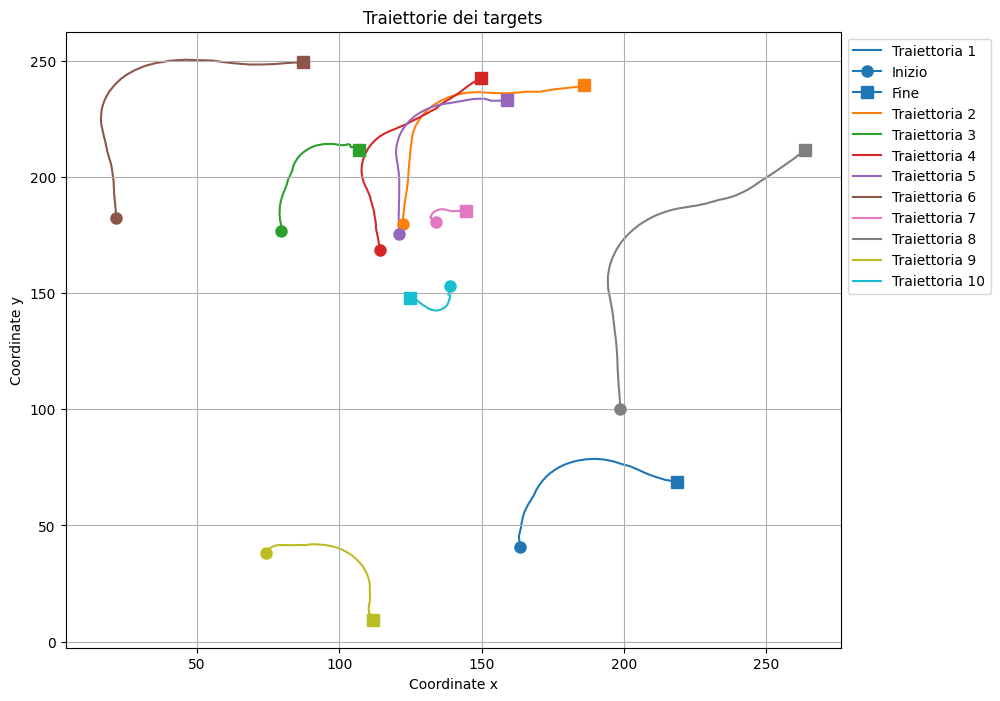
\includegraphics[width=1\textwidth]{Images/selectedTrajectories.png}
    \centering
    \caption{Traiettorie dei targets}
    \label{fig: traiettorieTargets}
\end{figure}
    

\vspace{\baselineskip}

2) \texttt{Generazione posizioni iniziale degli agenti}\\
Le posizioni iniziali degli agenti, essendo quattro, sono distribuite come segue:

\begin{itemize}
    \item Agente 1: $x = 50.0$, $y = 50.0$
    \item Agente 2: $x = 50.0$, $y = 150.0$
    \item Agente 3: $x = 150.0$, $y = 50.0$
    \item Agente 4: $x = 150.0$, $y = 150.0$
\end{itemize}

\begin{figure}[H]
    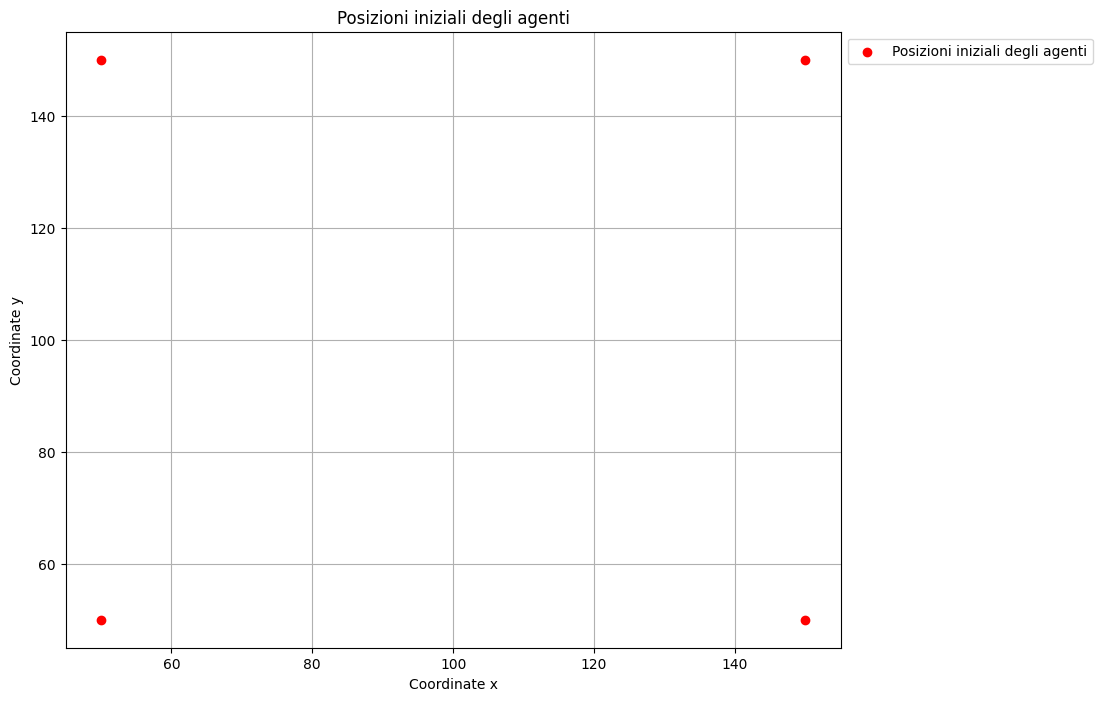
\includegraphics[width=0.8\textwidth]{Images/initialAgentPositions.png}
    \centering
    \caption{Posizioni inziali degli agenti}
    \label{fig: posInizAgenti}
\end{figure}

Per fornire una visione d'insieme, è incluso un grafico che mostra le traiettorie degli agenti insieme alle posizioni iniziali dei target. Si può osservare che gli agenti partono da posizioni prossime ai punti di partenza dei target, facilitando l'inizio dell'operazione di copertura.

\begin{figure}[H]
    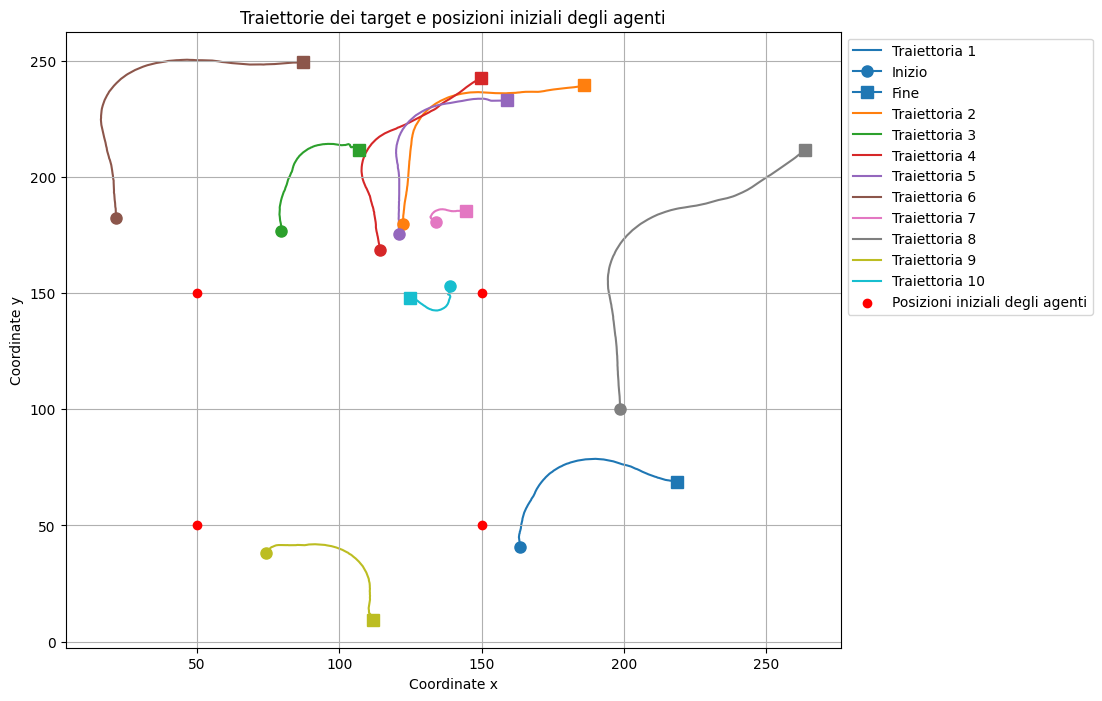
\includegraphics[width=1\textwidth]{Images/trajectoriesWithAgentStartPoints.png}
    \centering
    \caption{Traiettorie dei targets e posizioni iniziali degli agenti}
    \label{fig: targets&posInizAgenti}
\end{figure}

\vspace{\baselineskip}

3) \texttt{Calcolo degli indici di copertura iniziali}\\
Il calcolo degli indici di copertura iniziali è essenziale per confrontare i valori finali e valutare l'efficacia dell'algoritmo nell'incrementare la copertura.

\begin{table}[h]
\centering
\begin{tabular}{cc}
\toprule
$j$ & \(E_j(0)\) \\
\midrule
0 & 1.36690753 \\
1 & 1.43775742 \\
2 & 1.48737943 \\
3 & 1.64403469 \\
4 & 1.50434003 \\
5 & 0.92326174 \\
6 & 1.36251576 \\
7 & 1.22878553 \\
8 & 1.69180094 \\
9 & 1.71275626 \\
\bottomrule
\end{tabular}
\caption{Indici di copertura iniziali \(E_j(t)\) al tempo \(t=0\)}
\end{table}

Come si evince dalla tabella, al tempo iniziale \(t=0\), gli indici di copertura \(E_j(0)\) per tutti i target \(j\) sono in media superiori a 1. Ciò indica che inizialmente ogni target è coperto da poco più di un agente.

\vspace{\baselineskip}

Sotto viene riportato il valore iniziale dell'indice di copertura totale. Questo valore è fondamentale perché deve aumentare all'istante finale per dimostrare che la copertura dei target da parte degli agenti è migliorata.

\begin{table}[htbp]
\centering
\begin{tabular}{cccccccccc}
\toprule
$E(0)$ \\
\midrule
2.53832315 \\
\bottomrule
\end{tabular}
\caption{Valore iniziale dell'indice di copertura totale $E(0)$.}
\label{tab:indice_totale_iniziale}
\end{table}


\subsection{Analisi e grafici dei dati sperimentali}\label{section: analisiRisultati}

Dopo aver eseguito e testato le operazioni preliminari, si procede con l'implementazione delle tre versioni dell'algoritmo di copertura dinamica, oggetto di analisi del progetto. Questi algoritmi sono progettati per costruire le traiettorie degli agenti in modo tale che seguano correttamente i target e aumentino l'indice di copertura totale.\\
Di seguito i grafici completi che includono sia le traiettorie dei targets che quelle degli agenti, calcolate grazie all'esecuzione degli algoritmi:

\begin{figure}[H]
    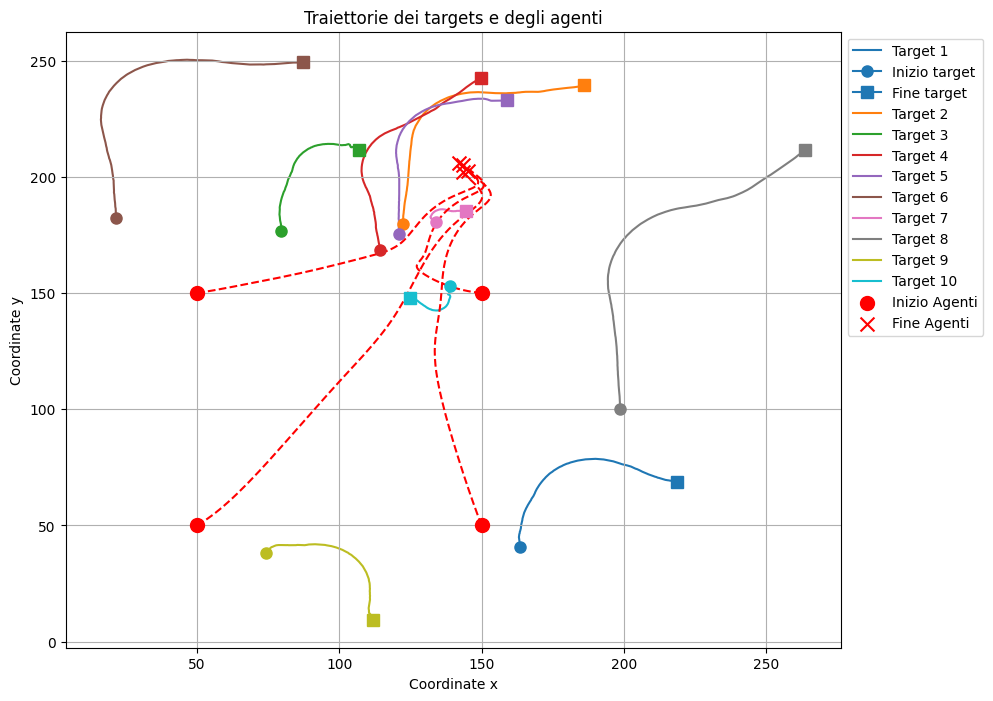
\includegraphics[width=0.9\textwidth]{Images/finalTrajectoriesV1.png}
    \centering
    \caption{Traiettorie dei targets e degli agenti, V1}
    \label{fig: traiettorieV1}
\end{figure}

\begin{figure}[H]
    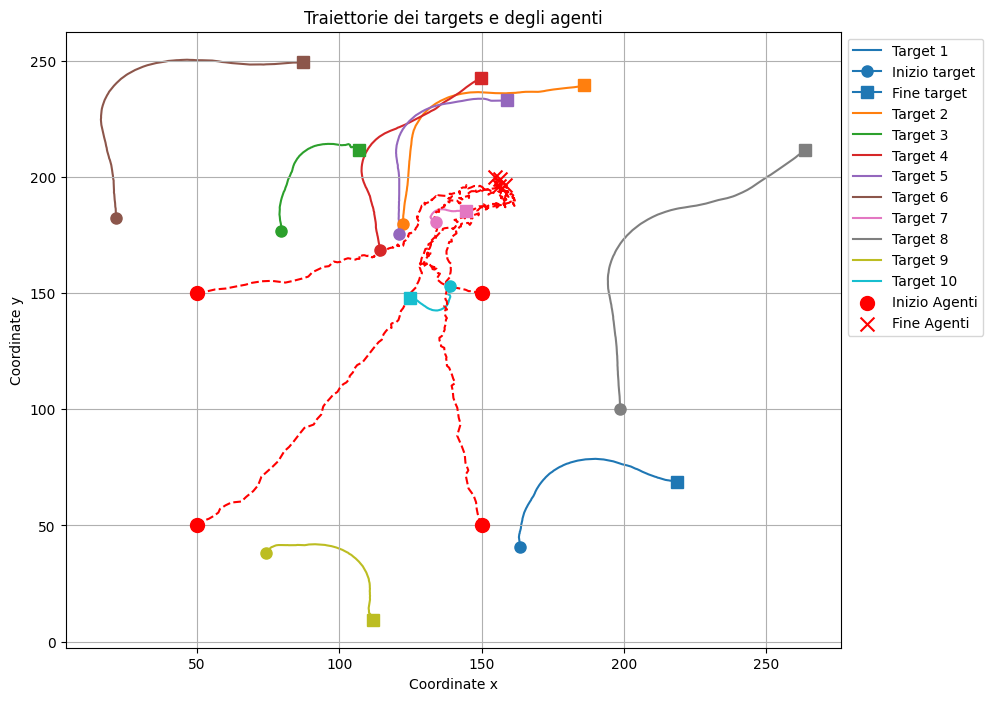
\includegraphics[width=0.9\textwidth]{Images/finalTrajectoriesV2.png}
    \centering
    \caption{Traiettorie dei targets e degli agenti, V2}
    \label{fig: traiettorieV2}
\end{figure}

\begin{figure}[H]
    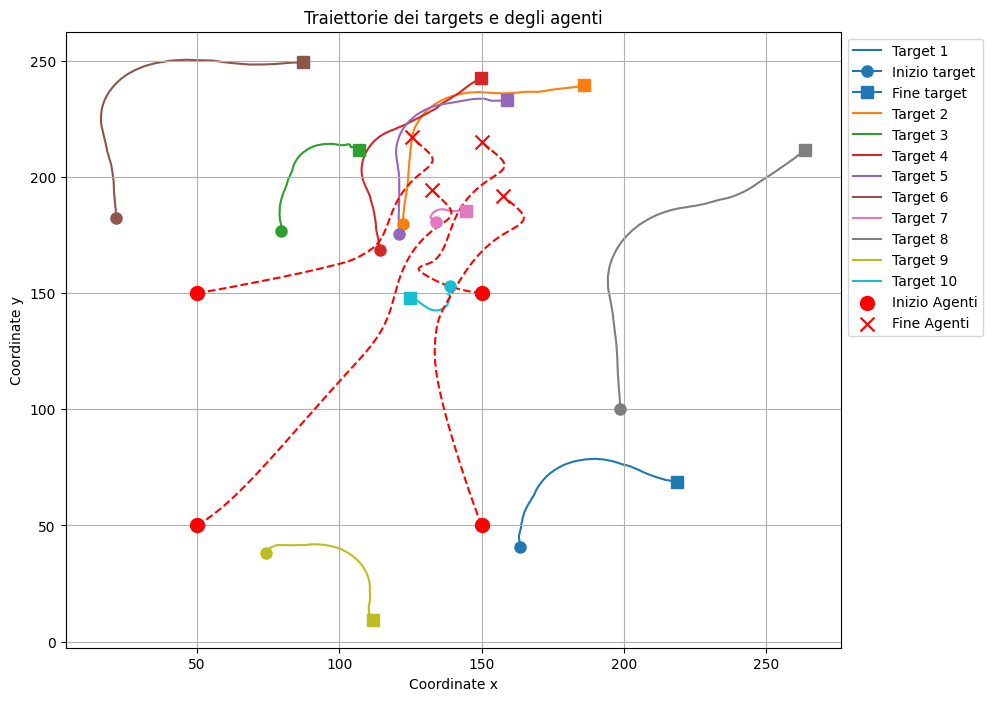
\includegraphics[width=0.9\textwidth]{Images/finalTrajectoriesV3.png}
    \centering
    \caption{Traiettorie dei targets e degli agenti, V3}
    \label{fig: traiettorieV3}
\end{figure}

Dai grafici delle traiettorie complete dei target e degli agenti (figure \ref{fig: traiettorieV1}, \ref{fig: traiettorieV2} e \ref{fig: traiettorieV3}) per le tre versioni dell'algoritmo, si può osservare che:

\begin{enumerate}
    \item Nella prima versione dell'algoritmo, descritta nella sezione \ref{section: v1}, i target finiscono per \textit{\textbf{collidere}} mentre cercano di massimizzare l'indice di copertura totale.
    \item Nella seconda versione, il problema della collisione non viene risolto in modo soddisfacente. Sebbene l'aggiunta del moto Browniano introduca variazioni casuali nelle traiettorie, i target tendono comunque a rimanere troppo vicini, finendo spesso in collisione.
    \item Nell'ultima versione, grazie all'introduzione del potenziale repulsivo, che entra in azione quando i target si avvicinano oltre una certa distanza \(\delta\), il problema della collisione viene efficacemente risolto. Questo risultato viene ottenuto senza compromettere la massimizzazione dell'indice di copertura totale, un aspetto che verrà analizzato più in dettaglio successivamente.
\end{enumerate}

Per determinare se l'obiettivo del progetto è stato raggiunto, è necessario effettuare un confronto tra gli indici di copertura iniziali e finali e trarre delle conclusioni in merito.\\
Di seguito sono riportati i grafici che illustrano l'andamento degli indici di copertura calcolati per tutte e tre le versioni dell'algoritmo.

\begin{figure}[H]
    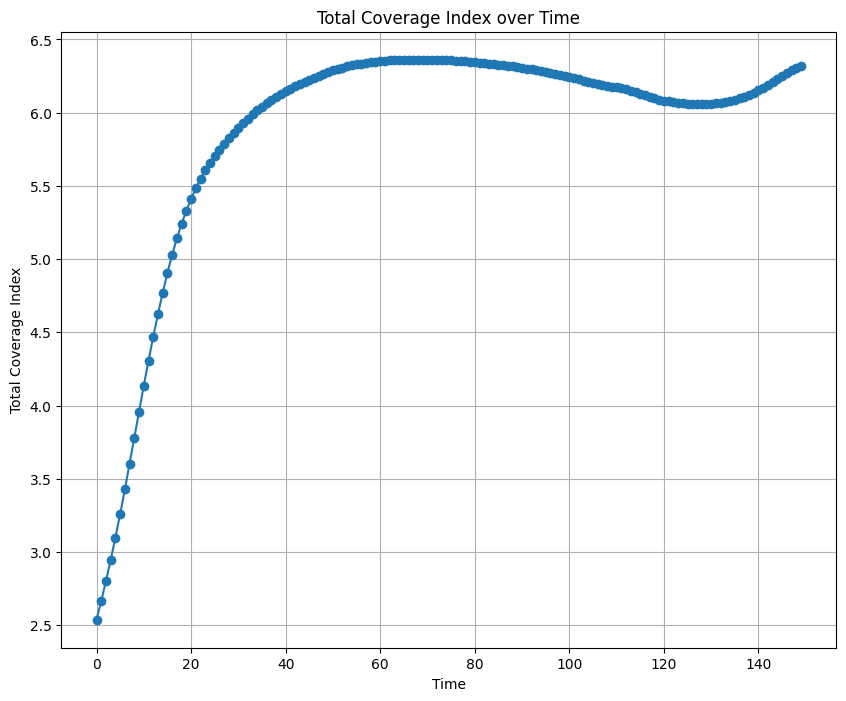
\includegraphics[width=0.7\textwidth]{Images/V1_totalCoverageIndexOverTime.png}
    \centering
    \caption{Indice di copertura totale $E(t)$, V1}
    \label{fig: indiceV1}
\end{figure}

\begin{figure}[H]
    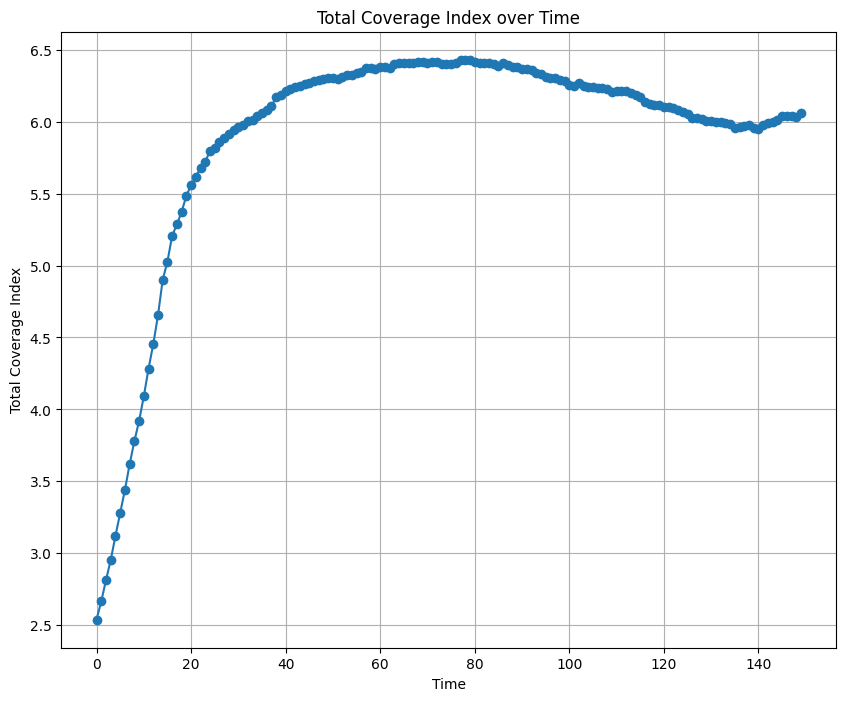
\includegraphics[width=0.7\textwidth]{Images/V2_totalCoverageIndexOverTime.png}
    \centering
    \caption{Indice di copertura totale $E(t)$, V2}
    \label{fig: indiceV2}
\end{figure}

\begin{figure}[H]
    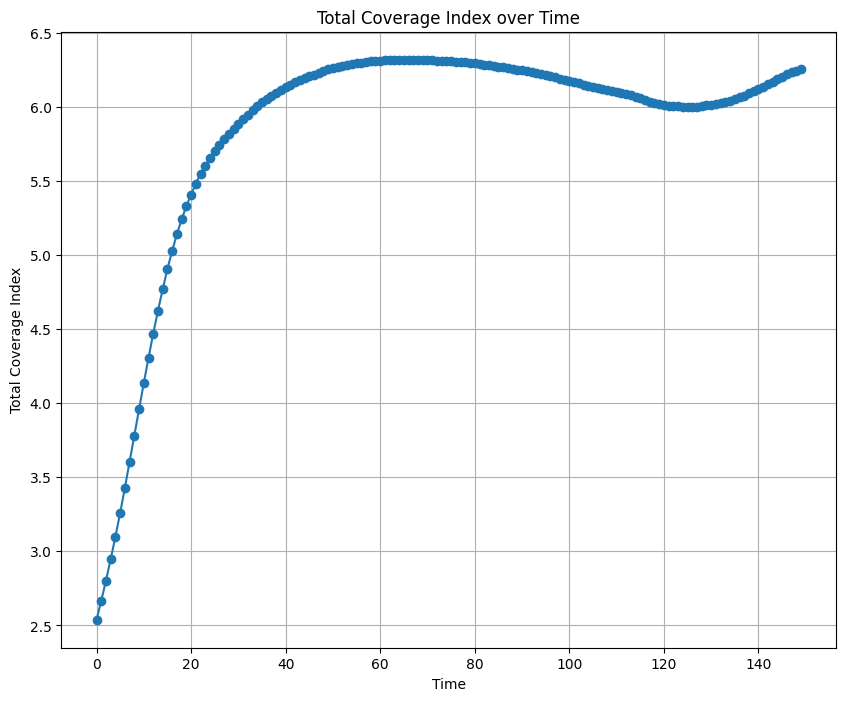
\includegraphics[width=0.7\textwidth]{Images/V3_totalCoverageIndexOverTime.png}
    \centering
    \caption{Indice di copertura totale $E(t)$, V3}
    \label{fig: indiceV3}
\end{figure}

Analizziamo anchei valori inziali e finali di questi tre diversi indici di copertura:

\begin{table}[H]
\centering
\begin{tabular}{cccc}
\toprule
 & \textbf{Valore Iniziale (E(0))} & \textbf{Valore Finale (E(duration-1))}\\ \midrule
\textbf{Algoritmo V1} & 2.5383 & 6.3206\\
\textbf{Algoritmo V2} & 2.5383 & 6.3725\\
\textbf{Algoritmo V3} & 2.5383 & 6.2578\\ \bottomrule
\end{tabular}
\caption{Confronto tra i valori iniziali e finali dell'indice di copertura totale}
\label{tab:confronto_indici}
\end{table}

Grazie all'analisi dei grafici e alla tabella di confronto, è possibile confermare che il progetto è stato portato a termine con successo e che gli algoritmi di coverage dinamico implementati soddisfano pienamente le aspettative iniziali:

\begin{enumerate}
    \item L'andamento del grafico dell'indice di copertura totale è crescente in tutte e tre le versioni dell'algoritmo. Il valore finale è significativamente maggiore rispetto al valore iniziale, indicando un notevole miglioramento nella copertura totale dell'area.
    
    \item I valori degli indici di copertura finali per le versioni 2 e 3 dell'algoritmo sono molto simili a quelli della versione originale. Questo risultato dimostra che la versione 3 dell'algoritmo è riuscita a evitare la collisione finale degli agenti, pur mantenendo un'elevata copertura dell'area e massimizzando l'indice di copertura. Questo aspetto conferma l'efficacia del metodo del potenziale repulsivo, descritto nella sezione \ref{section: v3}.
\end{enumerate}

\newpage

Per concludere, è importante andare anche ad analizzare il comportamento dei singoli indici di copertura dei target:

\begin{table}[H]
\centering
\begin{tabular}{ccccc}
\toprule
\textbf{Target j} & \textbf{Iniziale} & \textbf{Finale V1} & \textbf{Finale V2} & \textbf{Finale V3} \\
 & \(E_j(0)\) & \(E_j(150)\) & \(E_j(150)\) & \(E_j(150)\) \\
\midrule
\(j=0\) & 1.3669 & 0.0000 & 0.0038 & 0.0264 \\
\(j=1\) & 1.4378 & 2.9858 & 3.3193 & 2.8690 \\
\(j=2\) & 1.4874 & 3.5171 & 3.1065 & 3.4770 \\
\(j=3\) & 1.6440 & 3.4701 & 3.4722 & 3.3872 \\
\(j=4\) & 1.5043 & 3.6248 & 3.7138 & 3.5210 \\
\(j=5\) & 0.9233 & 2.3512 & 1.8834 & 2.3811 \\
\(j=6\) & 1.3625 & 3.8787 & 3.8085 & 3.7653 \\
\(j=7\) & 1.2288 & 0.5045 & 1.0068 & 0.4871 \\
\(j=8\) & 1.6918 & 0.0000 & 0.0000 & 0.0000 \\
\(j=9\) & 1.7128 & 2.8539 & 2.6135 & 2.7741 \\
\bottomrule
\end{tabular}
\caption{Confronto degli indici di copertura iniziali e finali per le tre versioni dell'algoritmo}
\label{tab:confronto-indici-copertura}
\end{table}

Come è possibile osservare dalla differenza tra i valori iniziali e quelli finali, la tesi analizzata nella sezione \ref{section: soluzioniProposte} è confermata. Inizialmente, ogni target è coperto in media da poco più di un agente, poiché gli indici iniziali sono leggermente superiori a 1 (si veda il ragionamento sui parametri analizzato in \ref{section: settingParametriIniziali}). Tuttavia, in tutte e tre le versioni, all'istante finale, gli indici di copertura del target 1 (j=0) e del target 9 (j=8) sono praticamente azzerati. Questo comportamento non è indesiderato, poiché l'algoritmo di copertura punta a massimizzare l'indice di copertura globale. Se per raggiungere questo obiettivo è necessario sacrificare alcuni target riducendo drasticamente la loro copertura, l'algoritmo lo fa. Questo comportamento può essere verificato osservando i grafici \ref{fig: traiettorieV1}, \ref{fig: traiettorieV2} e \ref{fig: traiettorieV3}, in cui si nota che i target azzurro e verdolino, nelle loro posizioni finali, sono molto distanti dalle posizioni finali degli agenti, addirittura fuori dal loro raggio di copertura. Gli agenti, seguendo la logica dell'algoritmo, tenderanno a concentrarsi nelle posizioni con una maggiore densità di target, al fine di massimizzare la funzione obiettivo, ovvero l'indice di copertura totale \textbf{(vedi figura \ref{fig: graficoFinale})}. \textit{Inoltre, solo 2 dei 10 target sono coperti in modo non soddisfacente, un risultato che risulta più che accettabile}.

\vspace{\baselineskip}

È importante notare anche che i valori degli \textit{\textbf{indici di copertura finali}} della maggior parte dei target sono nettamente superiori al valore di soglia \ensuremath{E*} pari a 2. Questo indica che i suddetti target avranno una copertura finale eccellente, confermando quanto affermato nella sezione \ref{section: soluzioniProposte}.

\vspace{\baselineskip}

Inoltre, i valori degli indici di copertura finali nelle tre diverse versioni dell'algoritmo di coverage sono piuttosto simili. Questo comportamento indica che, nonostante l'aggiunta di un moto browniano (\ref{section: v2}) o di un potenziale repulsivo (\ref{section: v3}), la qualità dell'algoritmo non è stata compromessa, mantenendo il trend principale dell'ascesa del gradiente. Nella versione 2, i cambiamenti dei valori rispetto alla versione classica sono molto casuali, dovuti alle componenti stocastiche del moto. Nella versione 3, invece, i valori sono leggermente inferiori, a favore però della non collisione finale degli agenti.

\begin{figure}[H]
    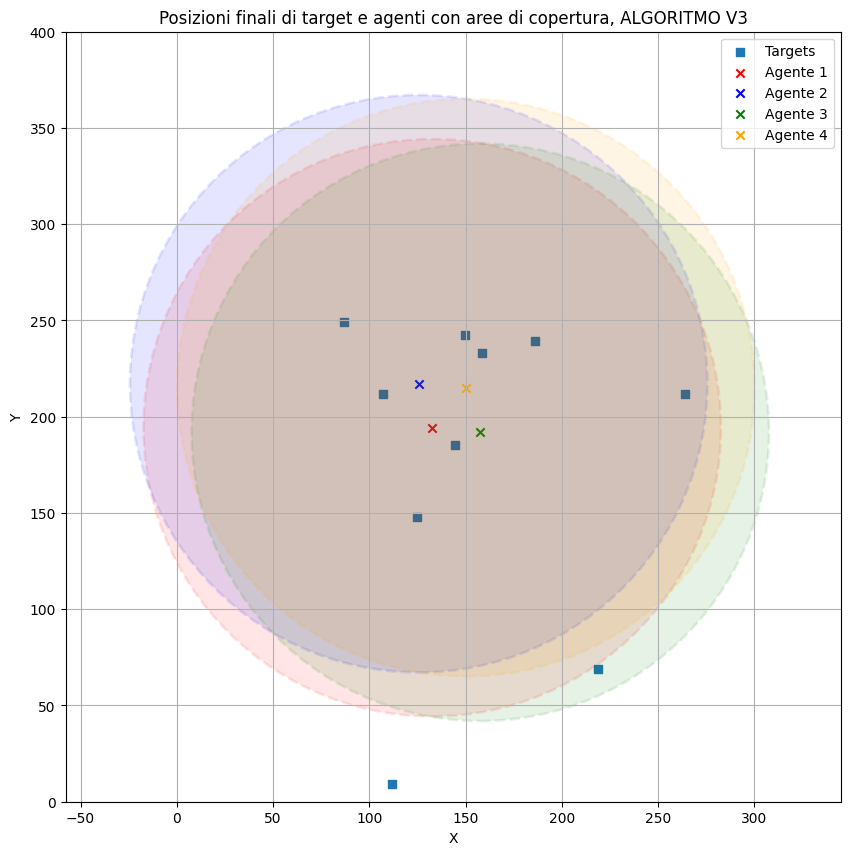
\includegraphics[width=0.8\textwidth]{Images/finalSetWithRadius.png}
    \centering
    \caption{Posizioni finali di targets e agenti con raggi di copertura}
    \label{fig: graficoFinale}
\end{figure}

Come ultima e importante conferma, il grafico che mostra le posizioni finali dei target e degli agenti con il loro raggio di copertura (traiettorie ottenute con la versione 3 dell'algoritmo) evidenzia che i target 1, 5 e 9 sono quelli coperti peggio. Confrontando questo grafico con la tabella \ref{tab:confronto-indici-copertura}, \textit{si può affermare che i dati e i risultati ottenuti sono coerenti con le aspettative teoriche}:

\begin{enumerate}
    \item Il target 9 (j=0) è completamente fuori dai raggi di copertura degli agenti; infatti, l'indice finale è sempre pari a 0 in tutte e tre le versioni.
    \item Il target 1 (j=1) è completamente fuori dai raggi di copertura nella prima versione dell'algoritmo, dove l'indice è pari a 0. Nelle altre due versioni è coperto in minima parte dal terzo agente, con un indice di copertura leggermente superiore a 0.
    \item Il target 6 (j=5) è coperto in modo meno efficiente rispetto agli altri. Tuttavia, il suo indice di copertura è mediamente superiore alla soglia \ensuremath{E* = 2}.
\end{enumerate}

\newpage



\subsection{Richiesta di coverage meno restrittiva}

\vspace{-30mm}

In questa sottosezione sarà analizzato il caso in cui il parametro \ensuremath{E* = lowerBoundIndex} è impostato a 1 anziché a 2. Questo implica una \textit{\textbf{richiesta di copertura inferiore}}: non è più necessario che almeno due agenti, in media, coprano un target, ma è sufficiente che sia coperto da un solo agente (vedi anche la sezione \ref{section: soluzioniProposte}).\\
Verranno esaminate tutte le conseguenze di questa scelta, replicando le considerazioni effettuate per il caso con \ensuremath{E* = 2} e confrontandole con quest'ultimo scenario.

\vspace{-10mm}

Considerando le operazioni preliminari già eseguite, le traiettorie dei targets e degli agenti, ottenute dopo l'esecuzione del codice, sono illustrate nei seguenti grafici per tutte e tre le versioni dell'algoritmo:

\FloatBarrier

\begin{figure}[H]
    \centering
    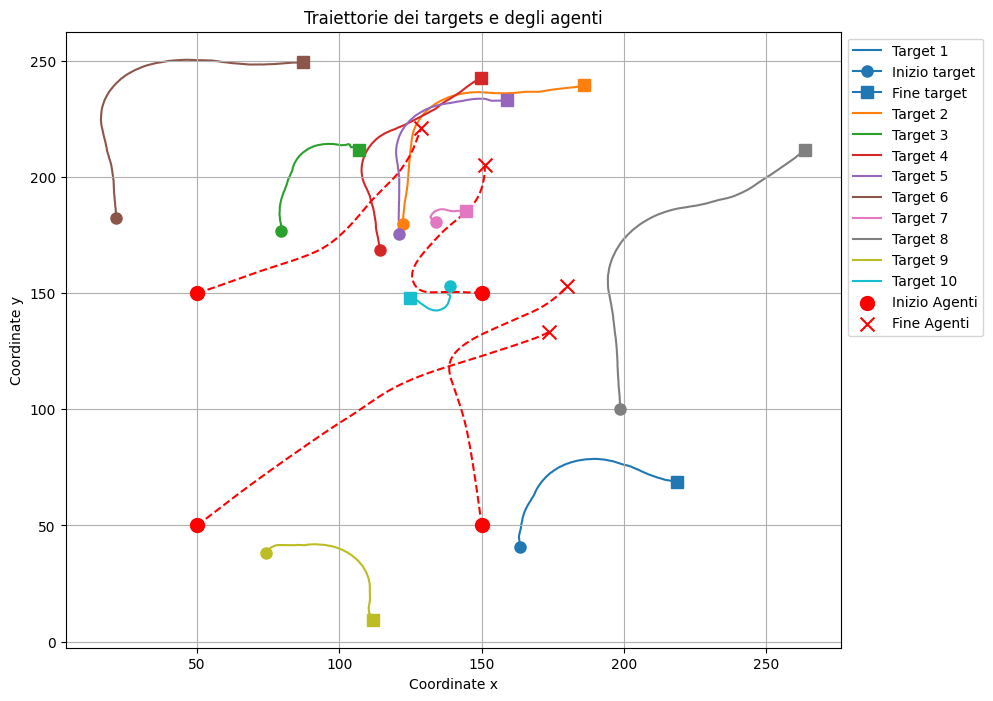
\includegraphics[width=0.9\textwidth]{Images/MP1_finalTrajectoriesV1.png}
    \caption{Traiettorie dei targets e degli agenti, V1, E*=1}
    \label{fig: MP1_traiettorieV1}
\end{figure}

\begin{figure}[H]
    \centering
    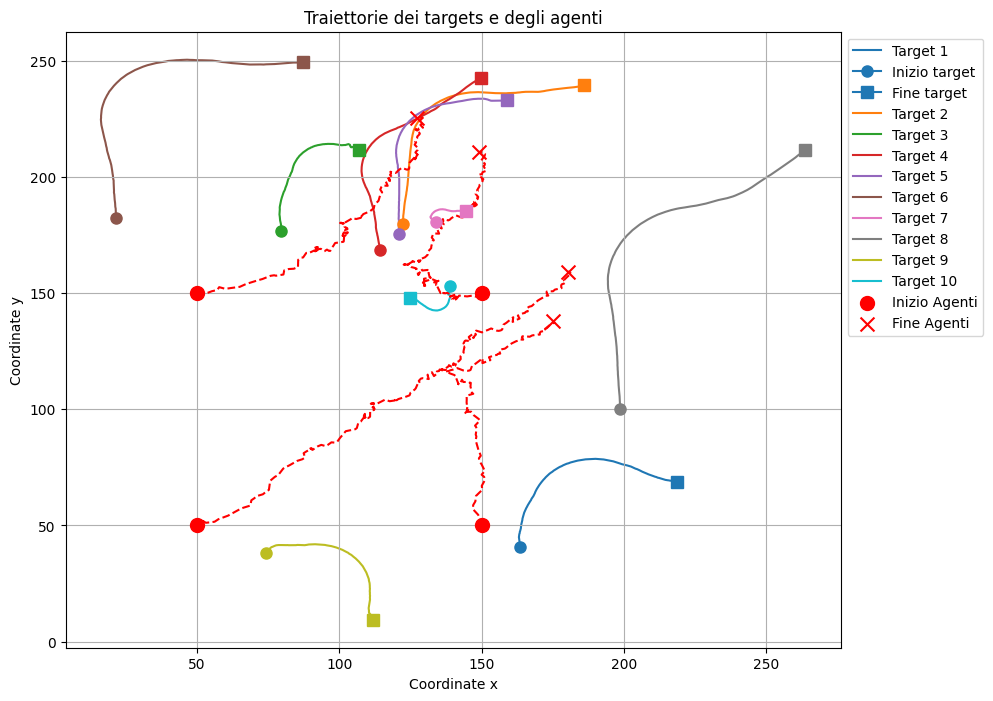
\includegraphics[width=0.9\textwidth]{Images/MP1_finalTrajectoriesV2.png}
    \caption{Traiettorie dei targets e degli agenti, V2, E*=1}
    \label{fig: MP1_traiettorieV2}
\end{figure}

\begin{figure}[H]
    \centering
    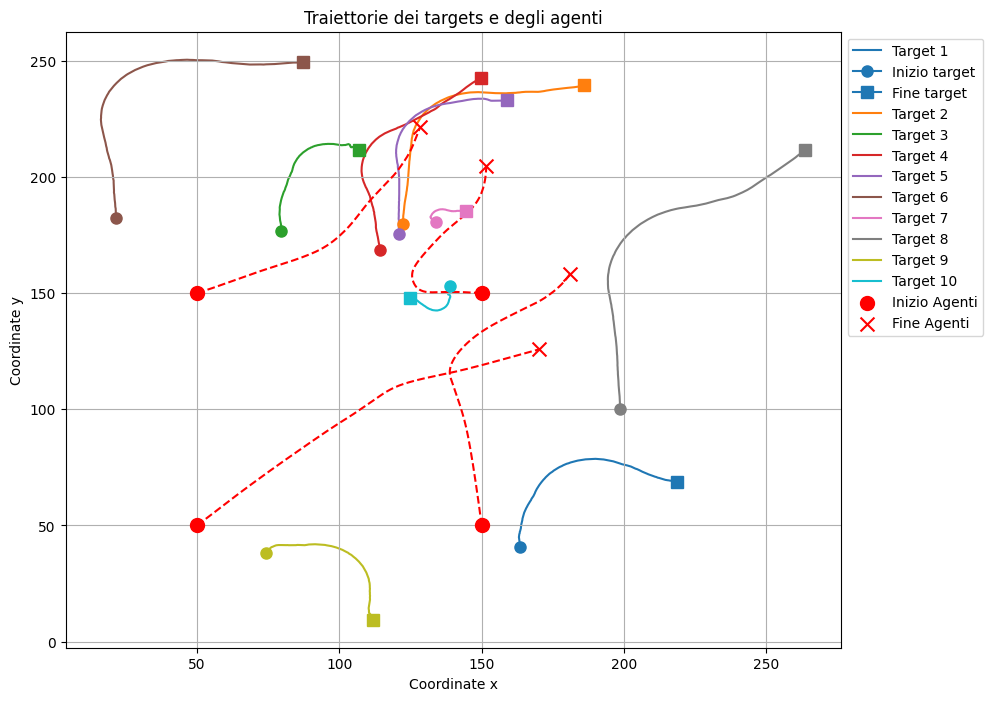
\includegraphics[width=0.9\textwidth]{Images/MP1_finalTrajectoriesV3.png}
    \caption{Traiettorie dei targets e degli agenti, V3, E*=1}
    \label{fig: MP1_traiettorieV3}
\end{figure}

\FloatBarrier

\vspace{\baselineskip}

Come si evince dalle figure \ref{fig: MP1_traiettorieV1}, \ref{fig: MP1_traiettorieV2} e \ref{fig: MP1_traiettorieV3}, a differenza dei grafici generati con \ensuremath{E*} impostato a 2 (figure \ref{fig: traiettorieV1}, \ref{fig: traiettorieV2} e \ref{fig: traiettorieV3}), emerge una notevole differenza: le posizioni finali degli agenti risultano significativamente diverse e molto più distanti tra loro.\\
Questo comportamento è perfettamente logico e conferma l'importanza del parametro \ensuremath{E*}. Con \ensuremath{E*} impostato alla metà del suo valore precedente, la richiesta di copertura è ridotta. Di conseguenza, è naturale che gli agenti non si avvicinino fino alla collisione. Dato che è necessario coprire i target con minore intensità, gli agenti possono permettersi di rimanere più distanti tra loro. Questo permette una copertura leggermente inferiore per i target precedentemente ben coperti e una copertura migliorata per i target che prima erano completamente fuori dal raggio di visione degli agenti, garantendo comunque una copertura complessivamente soddisfacente.\\
A conferma di questa tesi, si può osservare il grafico delle posizioni finali degli agenti e dei target, che mostra anche i raggi di copertura dei droni, e confrontarlo con il grafico precedente (\ref{fig: graficoFinale}):

\begin{figure}[H]
    \centering
    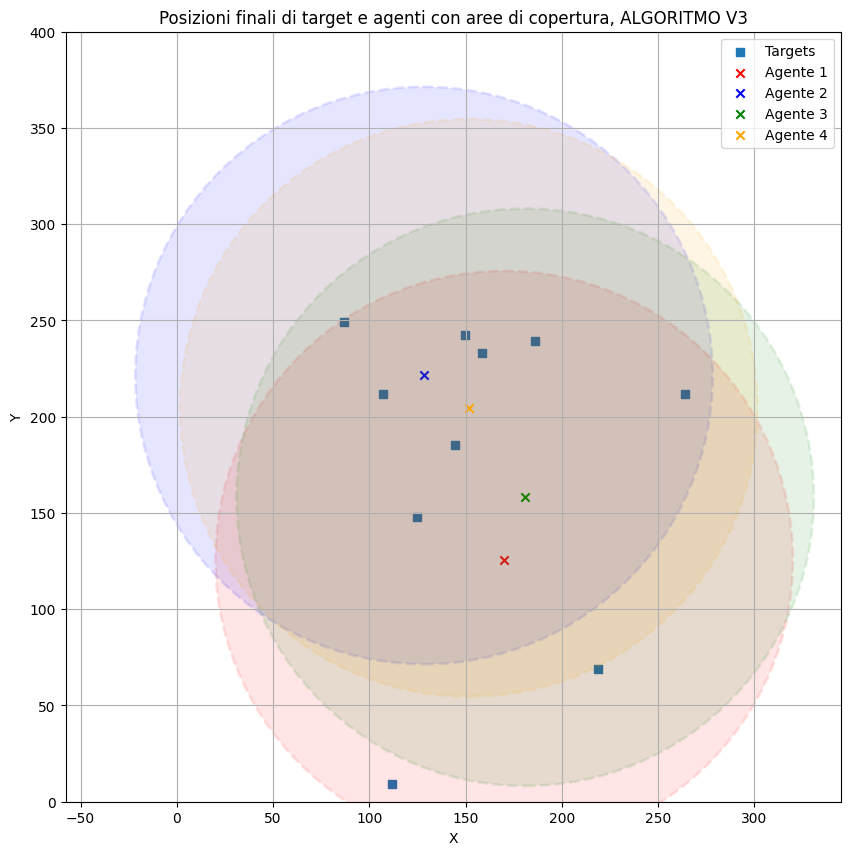
\includegraphics[width=1\textwidth]{Images/MP1_finalSetWithRadius.png}
    \caption{Posizioni finali di targets e agenti con raggi di copertura, E*=1}
    \label{fig: graficoFinale_E*=1}
\end{figure}

È fondamentale esaminare anche le differenze nei valori dei singoli indici di copertura e dell'indice di copertura totale:

\begin{table}[H]
\centering
\begin{tabular}{ccccc}
\toprule
\textbf{Target j} & \textbf{Iniziale} & \textbf{Finale V1} & \textbf{Finale V2} & \textbf{Finale V3} \\
 & \(E_j(0)\) & \(E_j(150)\) & \(E_j(150)\) & \(E_j(150)\) \\
\midrule
\(j=0\) & 1.3669 & 0.9107 & 0.9730 & 0.9051 \\
\(j=1\) & 1.4378 & 2.1927 & 2.1866 & 2.1717 \\
\(j=2\) & 1.4874 & 2.4315 & 2.3223 & 2.4179 \\
\(j=3\) & 1.6440 & 2.3590 & 2.3009 & 2.3455 \\
\(j=4\) & 1.5043 & 2.6228 & 2.5759 & 2.5999 \\
\(j=5\) & 0.9233 & 1.3669 & 1.2959 & 1.3758 \\
\(j=6\) & 1.3625 & 3.3449 & 3.2869 & 3.3143 \\
\(j=7\) & 1.2288 & 0.6475 & 0.7223 & 0.6294 \\
\(j=8\) & 1.6918 & 0.0217 & 0.0209 & 0.0613 \\
\(j=9\) & 1.7128 & 2.7822 & 2.7140 & 2.7725 \\
\bottomrule
\end{tabular}
\caption{Confronto degli indici di copertura iniziali e finali per le tre versioni dell'algoritmo, E*=1}
\label{tab:confronto-indici-copertura-E*=1}
\end{table}

Come si può osservare, i valori degli indici di copertura sono inferiori rispetto a quelli riportati nella tabella \ref{tab:confronto-indici-copertura}. Questo risultato è coerente, poiché la copertura richiesta è minore. Come descritto in precedenza, la copertura fornita è eccellente (superiore a \ensuremath{E* = 1}) per quasi tutti i target, ad eccezione dei tre target che erano già parzialmente coperti. Tuttavia, anche questi target marginali ora godono di una copertura migliore, con indici vicini alla soglia di 1 (vantaggio principale di andare ad essere meno restrittivi nella richiesta del coverage). Infatti, si può osservare che già all'istante iniziale si ottiene praticamente una copertura completa, con indici di copertura quasi tutti superiori alla soglia.

\vspace{\baselineskip}
Ci sono delle differenze sostanziali anche per quanto riguarda l'andamento dell'indice di copertura totale:

\begin{table}[H]
\centering
\begin{tabular}{cccc}
\toprule
 & \textbf{Valore Iniziale (E(0))} & \textbf{Valore Finale (E(duration-1))}\\ \midrule
\textbf{Algoritmo V1} & 6.9778 & 7.3113\\
\textbf{Algoritmo V2} & 6.9778 & 7.3153\\
\textbf{Algoritmo V3} & 6.9778 & 7.3042\\ \bottomrule
\end{tabular}
\caption{Confronto tra i valori iniziali e finali dell'indice di copertura totale, E*=1}
\label{tab:confronto_indici_E*=1}
\end{table}

Giustamente, il valore iniziale dell'indice di copertura totale è maggiore rispetto a quello riportato nella tabella \ref{tab:confronto_indici}. Questo avviene perché, con una richiesta di copertura inferiore per i singoli target, la copertura totale iniziale risulta migliorata. Anche se l'indice di copertura totale aumenterà all'istante finale, questo incremento non sarà così drastico come nel caso precedente con la soglia pari a 2. Questa osservazione è confermata dai grafici seguenti:

\begin{figure}[H]
    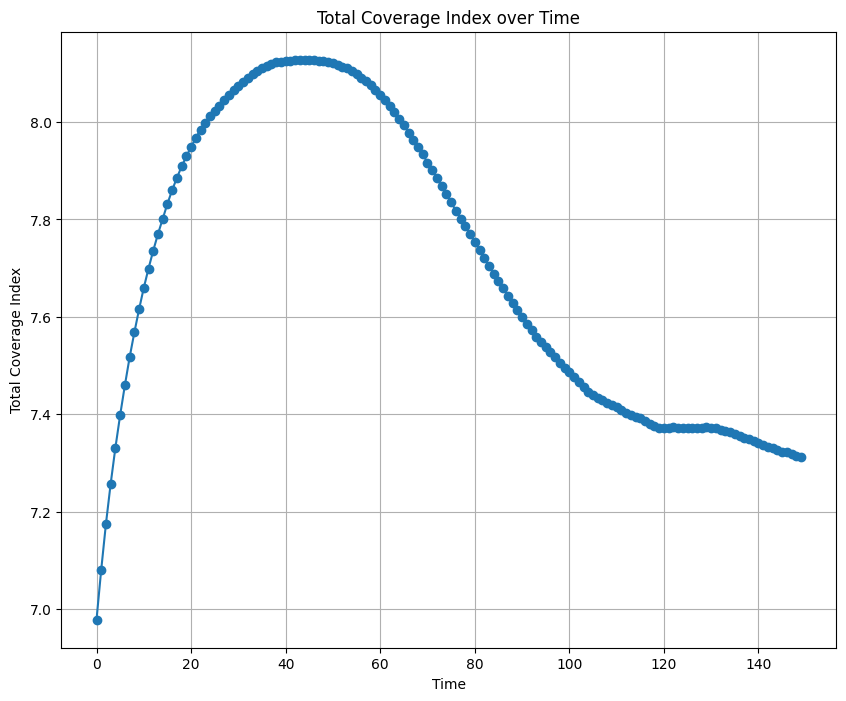
\includegraphics[width=0.8\textwidth]{Images/MP1_V1_totalCoverageIndexOverTime.png}
    \centering
    \caption{Indice di copertura totale $E(t)$, V1, E*=1}
    \label{fig: indiceV1_E*=1}
\end{figure}

\begin{figure}[H]
    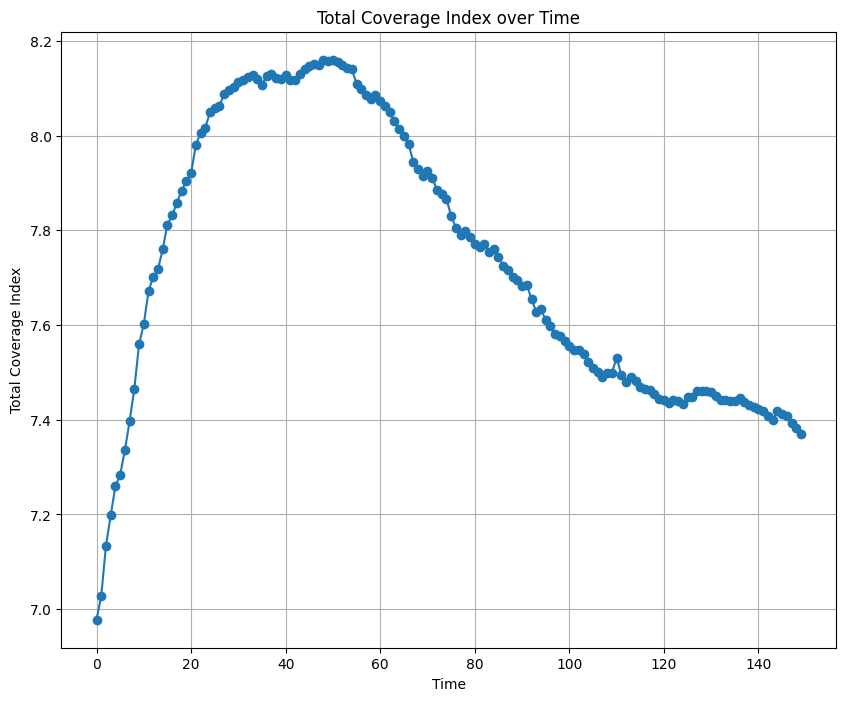
\includegraphics[width=0.8\textwidth]{Images/MP1_V2_totalCoverageIndexOverTime.png}
    \centering
    \caption{Indice di copertura totale $E(t)$, V2, E*=1}
    \label{fig: indiceV2_E*=1}
\end{figure}

\begin{figure}[H]
    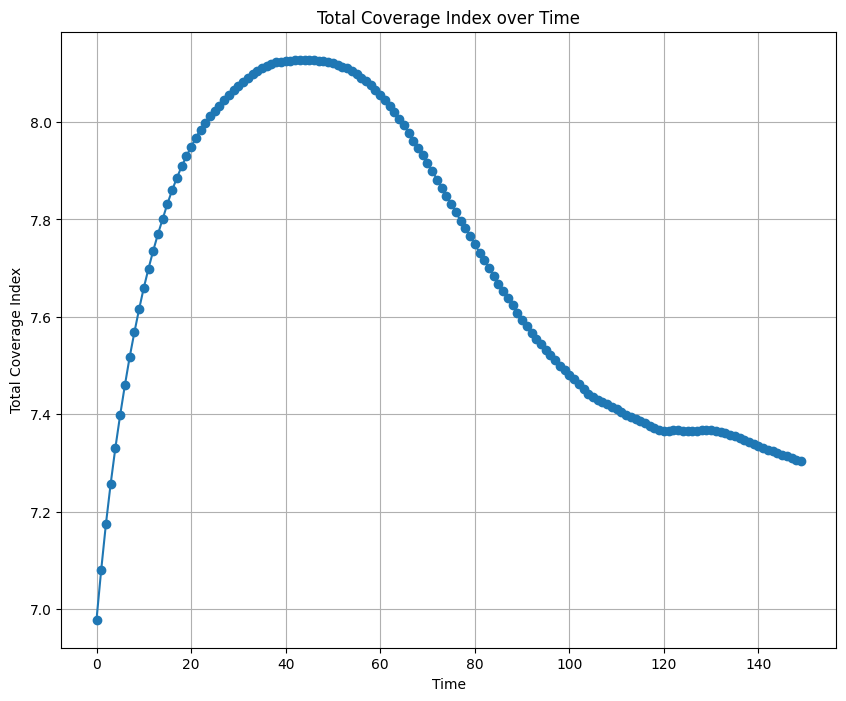
\includegraphics[width=0.8\textwidth]{Images/MP1_V3_totalCoverageIndexOverTime.png}
    \centering
    \caption{Indice di copertura totale $E(t)$, V3, E*=1}
    \label{fig: indiceV3_E*=1}
\end{figure}

Come evidenziato dai grafici precedenti, l'andamento dell'indice di copertura totale differisce rispetto al caso precedente. In questo scenario, si osserva una fase di crescita seguita da una fase di stabilizzazione. Nonostante ciò, il valore finale dell'indice di copertura totale risulta comunque superiore rispetto al caso con \ensuremath{E^* = 2}. Questo miglioramento della copertura totale è dovuto alla soglia inferiore. Pertanto, \textit{\textbf{è fondamentale comprendere il contesto specifico per trovare un compromesso ottimale tra il numero di target, il numero di agenti e la copertura richiesta}}.



% CONCLUSIONI------------------------------------------------------
\newpage
\addcontentsline{toc}{section}{Conclusioni}
\section*{\LARGE Conclusioni}

\vspace{\baselineskip}

In questa tesi di laurea, è stato affrontato il problema del controllo della copertura dinamica per il monitoraggio cooperativo in tempo reale utilizzando una flotta di agenti mobili. \textbf{Gli algoritmi sviluppati sono stati implementati e testati in un ambiente simulato, dimostrando la loro efficacia nel garantire un certo livello di copertura totale} fornito dagli agenti sui target dinamici.

\vspace{\baselineskip}

L'obiettivo primario di questi algoritmi è mantenere il più alto livello possibile di copertura totale per tutta la durata del monitoraggio, adattandosi dinamicamente ai cambiamenti nell'ambiente e nelle posizioni dei target. Gli algoritmi sono progettati per ottimizzare continuamente la copertura, cercando di aumentarla nel tempo e garantendo che il sistema multi-agente operi in modo efficiente e privo di collisioni.

\vspace{\baselineskip}

I risultati ottenuti confermano che tutti gli algoritmi sviluppati hanno migliorato significativamente l'indice di copertura totale rispetto allo stato iniziale. In particolare:

\begin{enumerate}
    \item La prima versione dell'algoritmo ha mostrato un notevole miglioramento dell'indice di copertura totale, ma ha presentato problemi di collisione tra gli agenti nelle posizioni finali.
    \item Nella seconda versione, l'introduzione del moto browniano ha mitigato parzialmente il problema delle collisioni, sebbene non in modo completamente soddisfacente.
    \item Nell'ultima versione, l'inclusione del potenziale repulsivo ha risolto efficacemente il problema delle collisioni senza compromettere l'aumento dell'indice di copertura totale, garantendo una distribuzione spaziale ottimale degli agenti.
\end{enumerate}

\vspace{\baselineskip}

\textbf{L'analisi dettagliata degli indici di copertura in funzione del tempo ha evidenziato che l'algoritmo riesce ad aumentare e garantire nel tempo un alto livello di copertura per i target che si muovono all'interno dell'area di sorveglianza.}

\vspace{\baselineskip}

Inoltre, è stato analizzato l'effetto della diminuzione della richiesta di copertura sull'indice di copertura totale. In particolare, con una richiesta di copertura inferiore, gli agenti possono distribuire le loro risorse in modo più efficiente, portando a un aumento complessivo dell'indice di copertura totale. Questa osservazione suggerisce che la flessibilità nella richiesta di copertura può condurre a una gestione più efficiente delle risorse degli agenti, migliorando ulteriormente la qualità del monitoraggio.

\vspace{\baselineskip}

In conclusione, i risultati di questa tesi dimostrano che gli algoritmi sviluppati forniscono una soluzione robusta ed efficace per il controllo della copertura dinamica, con potenziali applicazioni in numerosi campi, dalla sorveglianza alla gestione delle emergenze.

\newpage

Ecco una lista di alcuni \textbf{possibili sviluppi} di questa tesi di laurea:
\begin{enumerate}
    \item Un primo sviluppo futuro consiste nell'andare oltre l'approccio greedy basato su informazioni istantanee, integrando la predizione delle traiettorie dei target tramite tecniche avanzate come Reinforcement Learning (RL), Deep Reinforcement Learning (DRL), Multi-Agent Deep Reinforcement Learning (MADRL) e approcci model-based. Il RL permette agli agenti di apprendere politiche ottimali massimizzando le ricompense cumulative \cite{SuttonBarto2018}, mentre il DRL utilizza reti neurali profonde per apprendere in spazi di stato e azione continui \cite{Mnih2015}. Il MADRL estende questi concetti a scenari multi-agente, ottimizzando la cooperazione e la competizione tra agenti \cite{Lowe2017}. Gli approcci model-based costruiscono modelli delle transizioni di stato per migliorare la predizione delle dinamiche temporali e l'efficienza dell'apprendimento \cite{Chua2018}.
    
    \item Un secondo sviluppo futuro potrebbe riguardare la modifica dell'altitudine degli agenti, poiché nella progetto attuale essa è fissata. Un'alterazione dell'altitudine permette agli agenti di coprire un'area maggiore, se volano più in alto, ma a scapito di una risoluzione inferiore delle immagini o dei dati raccolti. La sfida risiede nel trovare un compromesso ottimale tra estensione dell'area coperta e qualità della risoluzione. Tecniche di ottimizzazione multi-obiettivo potrebbero essere impiegate per bilanciare questi due aspetti, garantendo che la copertura sia sufficientemente ampia senza compromettere eccessivamente la risoluzione dei dati \cite{Zhao2019}, \cite{Beard2020}. Questo approccio potrebbe essere ulteriormente migliorato integrando modelli predittivi che aiutino a decidere l'altitudine ottimale in tempo reale, in base alla dinamica dei target e alle esigenze di risoluzione \cite{Merino2006}.
    
    \item Un terzo possibile sviluppo riguarda l'esplorazione dell'area di interesse. Nel progetto di tesi, si assume di conoscere a priori il punto di partenza dei target, le loro traiettorie e il numero preciso di target presenti nella zona di analisi. Tuttavia, in scenari reali, queste informazioni potrebbero non essere disponibili. Pertanto, un'estensione del lavoro potrebbe consistere nell'integrare una fase di esplorazione, in cui gli agenti effettuano una ricognizione dell'area per raccogliere informazioni sulla posizione e sul numero dei target. Questa esplorazione potrebbe utilizzare tecniche di SLAM (Simultaneous Localization and Mapping) per mappare l'ambiente e individuare i target \cite{Thrun2005}, \cite{Cadena2016}.\\
    L'esplorazione non solo aiuterebbe a mappare l'area e a identificare i target, ma potrebbe anche rilevare la presenza di intrusi o oggetti non previsti. Metodi avanzati di esplorazione autonoma, basati su approcci di ottimizzazione e tecniche probabilistiche, possono migliorare l'efficienza e la precisione di questa fase \cite{Bircher2016}.
\end{enumerate}





% BIBLIOGRAFIA ----------------------------------------------------

\newpage

% Aggiungi la sezione "Bibliografia" all'indice senza visualizzarla
\phantomsection
\addcontentsline{toc}{section}{Bibliografia}

% Crea la sezione "Bibliografia" in \LARGE
%\section*{\LARGE Bibliografia}

\begin{thebibliography}{99}

\vspace{\baselineskip}

\bibitem{Articolo_0}
J. Cortes, S. Martinez, T. Karatas and F. Bullo, "Coverage control for mobile sensing networks," in IEEE Transactions on Robotics and Automation, vol. 20, no. 2, pp. 243-255, April 2004, doi: 10.1109/TRA.2004.824698.
keywords: {Sensor phenomena and characterization;Remotely operated vehicles;Mobile robots;Temperature sensors;Biosensors;Animals;Optimization methods;Partitioning algorithms;Prototypes;Infrared sensors},
\url{https://ieeexplore.ieee.org/document/1284411}

\bibitem{Articolo_1}
S. Meng and Z. Kan, "Deep Reinforcement Learning-Based Effective Coverage Control With Connectivity Constraints," in IEEE Control Systems Letters, vol. 6, pp. 283-288, 2022, doi: 10.1109/LCSYS.2021.3070850.
keywords: {Sensors;Monitoring;Dynamics;Task analysis;Reinforcement learning;Vehicle dynamics;Training;Coverage control;deep reinforcement learning;multi-agent systems},
\url{https://ieeexplore.ieee.org/document/9395182}

\bibitem{Articolo_2}
Hübel, Nico. (2008). Coverage Control with Information Decay in Dynamic Environments. IFAC Proceedings Volumes. 41. 4180-4185. 10.3182/20080706-5-KR-1001.00703. 
\url{https://www.researchgate.net/publication/254995455_Coverage_Control_with_Information_Decay_in_Dynamic_Environments}

\bibitem{LibroAscesaGradiente}
Goodfellow, I., Bengio, Y., Courville, A. (2016). Deep Learning. MIT Press.
\url{https://www.deeplearningbook.org/}

\bibitem{collisionAvoidance}
Stipanović, D.M., Hokayem, P.F., Spong, M.W., \& Šiljak, D.D. (2007). Cooperative avoidance control for multi-agent systems. \textit{Journal of Dynamic Systems, Measurement, and Control}, 129, 699-707. doi:10.1115/1.2764502.
\url{https://asmedigitalcollection.asme.org/dynamicsystems/article-abstract/129/5/699/446752/Cooperative-Avoidance-Control-for-Multiagent}

\bibitem{StochasticProcesses}
E. Nelson, \textit{Dynamical Theories of Brownian Motion}, Princeton University Press, 1967.
\url{https://web.math.princeton.edu/~nelson/books/bmotion.pdf}

\bibitem{Abdechiri2013}
M. Abdechiri, M. R. Meybodi, H. Bahrami, \textit{Gases Brownian motion optimization: an algorithm for optimization (GBMO)}, Applied Soft Computing, 2013.\\
\url{https://www.sciencedirect.com/science/article/pii/S1568494612001834}

\bibitem{Sowjanya2021}
K. Sowjanya, S. K. Injeti, \textit{Investigation of butterfly optimization and gases Brownian motion optimization algorithms for optimal multilevel image thresholding}, Expert Systems with Applications, 2021.\\
\url{https://www.sciencedirect.com/science/article/pii/S095741742100717X}

\bibitem{Xiaohong2012}
Q. Xiaohong, Q. Xiaohui, \textit{An evolutionary particle swarm optimizer based on fractal Brownian motion}, Journal of Computational Intelligence, 2012.\\
\url{https://www.ingentaconnect.com/contentone/asp/jcies/2012/00000001/00000001/art00023}

\bibitem{MDPI_Hao}
H. Hao, et al., \textit{Potential Field Method for Multi-Agent Formation Control with Collision Avoidance}, MDPI, 2020.\\
\url{https://www.mdpi.com/2076-3417/10/20/7259}

\bibitem{MDPI_Jiang}
J. Jiang, et al., \textit{Enhanced Dynamic Coverage Using Repulsive Potentials in Multi-Agent Systems}, MDPI, 2021.\\
\url{https://www.mdpi.com/2079-9292/10/8/950}

\bibitem{Nagy2009}
I. Nagy, \textit{Behaviour Study of a Multi-Agent Mobile Robot System during Potential Field Building}, Acta Polytechnica Hungarica, 2009.\\
\url{https://www.researchgate.net/publication/45087275_Behaviour_Study_of_a_Multi-Agent_Mobile_Robot_System_during_Potential_Field_Building}

\bibitem{Arkin1994}
R. Arkin, K. Ali, \textit{Integration of Reactive and Telerobotic Control in Multi-Agent Robotic Systems}, Proc. Simulation of Adaptive Behavior, 1994.\\
\url{https://www-robotics.jpl.nasa.gov/media/documents/sab94.pdf}

\bibitem{Mabrouk2008}
M.H. Mabrouk, C.R. McInnes, \textit{Social Potential Model to Simulate Emergent Behaviour for Swarm Robots}, 13th International Conference on Climbing and Walking Robots, 2008.\\
\url{https://strathprints.strath.ac.uk/7528/6/strathprints007528.pdf}

\bibitem{Pickle}
\url{https://docs.python.it/html/lib/module-pickle.html}

\bibitem{Hoffman} Joe D. Hoffman, \textit{Numerical Methods for Engineers and Scientists}, 2nd Edition, CRC Press, 2001.\\
\url{https://www.crcpress.com/Numerical-Methods-for-Engineers-and-Scientists-Second-Edition/Hoffman/p/book/9780824704438}

\bibitem{Epperson} James F. Epperson, \textit{An Introduction to Numerical Methods and Analysis}, 2nd Edition, Wiley, 2013.\\
\url{https://www.wiley.com/en-us/An+Introduction+to+Numerical+Methods+and+Analysis%2C+2nd+Edition-p-9781118367599}

\bibitem{NumPyDocumentation} NumPy Developers, \textit{NumPy: The fundamental package for scientific computing with Python}, \url{https://numpy.org/doc/stable/}.

\bibitem{PickleDocumentation} Python Software Foundation, \textit{pickle - Python object serialization}, \url{https://docs.python.org/3/library/pickle.html}.

\bibitem{Hunter:2007}
John D. Hunter, \textit{Matplotlib: A 2D Graphics Environment}, 2007.
\url{https://matplotlib.org/stable/contents.html}

\bibitem{PyTorch} Adam Paszke, Sam Gross, Soumith Chintala, Gregory Chanan, Edward Yang, Zachary DeVito, Zeming Lin, Alban Desmaison, Luca Antiga, Adam Lerer. \textit{Automatic differentiation in PyTorch}, 2017. \url{https://pytorch.org}.

\bibitem{Cormen2009} T. H. Cormen, C. E. Leiserson, R. L. Rivest, and C. Stein, \textit{Introduction to Algorithms}, 3rd ed. MIT Press, 2009. \url{https://mitpress.mit.edu/books/introduction-algorithms-third-edition}

\bibitem{Kleinberg2006} J. Kleinberg and É. Tardos, \textit{Algorithm Design}. Pearson, 2006. \url{https://www.pearson.com/store/p/algorithm-design/P100000052280}

\bibitem{SuttonBarto2018} R. S. Sutton and A. G. Barto, \textit{Reinforcement Learning: An Introduction}. MIT press, 2018. \url{https://web.stanford.edu/class/psych209/Readings/SuttonBartoIPRLBook2ndEd.pdf}

\bibitem{Mnih2015} V. Mnih et al., "Human-level control through deep reinforcement learning," \textit{Nature}, vol. 518, no. 7540, pp. 529--533, 2015. \url{https://www.nature.com/articles/nature14236}

\bibitem{Lowe2017} R. Lowe et al., "Multi-agent actor-critic for mixed cooperative-competitive environments," \textit{Advances in Neural Information Processing Systems}, vol. 30, 2017. \url{https://proceedings.neurips.cc/paper/2017/file/68a9750337a418a86fe06c1991a1d64c-Paper.pdf}

\bibitem{Chua2018} K. Chua et al., "Deep reinforcement learning in a handful of trials using probabilistic dynamics models," \textit{Advances in Neural Information Processing Systems}, vol. 31, 2018. \url{https://proceedings.neurips.cc/paper/2018/file/3de568f8597b94bda53149c7d7f8b16c-Paper.pdf}

\bibitem{Zhao2019} Y. Zhao, L. Meng, and S. Wang, "Multi-objective optimization for coverage path planning in aerial remote sensing," \textit{IEEE Access}, vol. 7, pp. 45606-45619, 2019. \url{https://ieeexplore.ieee.org/document/8695680}

\bibitem{Beard2020} R. Beard and T. McLain, \textit{Small Unmanned Aircraft: Theory and Practice}. Princeton University Press, 2020. \url{https://press.princeton.edu/books/hardcover/9780691149219/small-unmanned-aircraft}

\bibitem{Merino2006} L. Merino, F. Caballero, J. R. Martínez-de-Dios, I. Maza, and A. Ollero, "A cooperative perception system for multiple UAVs: Application to automatic detection of forest fires," \textit{Journal of Field Robotics}, vol. 23, no. 3-4, pp. 165-184, 2006. \url{https://onlinelibrary.wiley.com/doi/abs/10.1002/rob.20109}

\bibitem{Thrun2005} S. Thrun, W. Burgard, and D. Fox, \textit{Probabilistic Robotics}. MIT Press, 2005. \url{https://mitpress.mit.edu/9780262201629/probabilistic-robotics/}

\bibitem{Cadena2016} C. Cadena, L. Carlone, H. Carrillo, Y. Latif, D. Scaramuzza, J. Neira, I. Reid, and J. J. Leonard, "Past, present, and future of simultaneous localization and mapping: Toward the robust-perception age," \textit{IEEE Transactions on Robotics}, vol. 32, no. 6, pp. 1309-1332, 2016. \url{https://doi.org/10.1109/TRO.2016.2624754}

\bibitem{Bircher2016} A. Bircher, M. Kamel, K. Alexis, H. Oleynikova, and R. Siegwart, "Receding horizon path planning for 3D exploration and surface inspection," \textit{Autonomous Robots}, vol. 42, pp. 291-306, 2016. \url{https://link.springer.com/article/10.1007/s10514-016-9549-1}

\end{thebibliography}


% RINGRAZIAMENTI --------------------------------------------------
\newpage
\addcontentsline{toc}{section}{Ringraziamenti}
\section*{\LARGE Ringraziamenti}

\vspace{\baselineskip}

\setstretch{1.5} % Modifica la spaziatura per rendere i ringraziamenti più leggibili

Questi anni di università sono stati caratterizzati da molti sacrifici, rinunce e momenti di sofferenza. Fortunatamente, queste difficoltà sono state sempre alleviate dalla presenza delle persone a me care. A tutti coloro che mi sono stati vicini, dico Grazie, dal cuore. Tuttavia, alcune persone meritano un ringraziamento particolare:

\vspace{\baselineskip}

\textit{Ai miei genitori,}\\
che, nonostante tutto, non mi hanno mai fatto mancare nulla. Nonostante i vari problemi familiari, mi hanno sempre dato la possibilità di fare ciò che desideravo, supportandomi nel bene e nel male. Grazie a loro, sono la persona forte di oggi. Mi hanno insegnato i valori della vita, tra cui l'educazione e la dedizione. Devono sapere che tutto ciò che faccio, tutto l'impegno che metto in ambito accademico e lavorativo, è per restituire loro, un giorno, tutto ciò che mi hanno dato, senza mai chiedere nulla in cambio.

\vspace{\baselineskip}

\textit{A Elia,}\\
per essere sempre stato vicino a me, nonostante il mio carattere molto particolare.

\vspace{\baselineskip}

\textit{A mio cugino Matteo,}\\
per essere il mio più grande punto di riferimento da sempre. Quando penso di non farcela, mi ricordo quanto è intelligente e mi motivo, cercando di diventare migliore di lui (è impossibile).

\vspace{\baselineskip}

\textit{Alle mie carissime nonne,}\\
per avermi sempre detto che sono il più bravo di tutti, per avermi cucinato per tutta la mia vita, per avermi fatto passare i momenti più belli della mia infanzia.

\vspace{\baselineskip}

\textit{A Sara,}\\
per essere entrata nella mia vita e avermi dato così tanto in così poco. Lei mi supporta qualsiasi cosa io faccia, mi fa analizzare i vantaggi e gli svantaggi delle mie scelte, mi ha fatto maturare tanto e mi sta dando moltissimo affetto. Potrei spendere mille parole per ringraziarla. Le vorrei solo dire che per me contano le piccole cose, come quando mi accompagna ad ogni mia gara, mi prepara da mangiare esattamente come lo voglio io e fa di tutto pur di farmi stare tranquillo. Non immagina quanto apprezzo e noto queste cose. Mi difende sempre e soprattutto mi aiuta ad affrontare i momenti difficili che magari, senza di lei, non riuscirei a superare.

\vspace{\baselineskip}

\textit{A Nicco,}\\
per essere un mio grande amico e un grande punto di riferimento. Con lui mi sono fatto le più grandi risate della mia vita. Deve sapere che ogni goccia di sudore che ho versato in questo periodo è stata per mantenere una promessa: sto arrivando a Torino.

\vspace{\baselineskip}

\textit{A Dani,}\\
perché il nostro rapporto è impossibile da descrivere a parole. Non penso sia suo volere che io spenda troppe parole per ringraziarlo, dato che passiamo già tanto tempo a discutere di argomenti che pochi ragazzi della nostra età affrontano. Tuttavia, una cosa mi sento di dirla: gli auguro il meglio e che tutti i momenti difficili che ha vissuto lo portino a raggiungere i suoi obiettivi. Io ci sarò sempre per lui.

\vspace{\baselineskip}

\textit{A Matti,}\\
perché ciò che abbiamo passato e creato insieme non ha eguali. Sono cresciuto e maturato con lui, realizzando i miei sogni insieme a lui. Spero che le nostre strade non si dividano mai, e ne sono convinto, perché il legame che abbiamo è come quello di una famiglia.

\vspace{\baselineskip}

\textit{A Kri,}\\
perché per primo ha creduto nei sogni miei e di Mattia, è stata la prima persona che ci ha dato tutta la sua passione e la sua fiducia. Sono sicuro che su di lui posso contare.

\vspace{\baselineskip}

\textit{Alla mia amica Giorgia,}\\
perchè in questi anni è stata la persona da battere, in senso buono. È stata l'unica persona che, quando dovevo preparare la tesi e l'esame di Fisica 2 in sole tre settimane, si è messa a buttare giù delle idee mentre camminava, creando un vero e proprio piano di studio che nessun'altra persona al mondo potrebbe neanche sognarsi di portare a termine. Lei, nel suo, è la più forte di tutti.

\vspace{\baselineskip}

\textit{Al Vernia,}\\
per esserci sempre, indipendentemente dal problema. Mi ispiro molto a lui per quello che fa, nonostante le varie tempeste che deve affrontare, persiste senza mai mollare. Ne abbiamo passate tante, e le abbiamo superate tutte con le nostre forze. Spero che un giorno possa realizzare tutti i suoi sogni.

\vspace{\baselineskip}
\vspace{\baselineskip}
\vspace{\baselineskip}

\textit{Al Sensei,}\\
per essere stato una vera e propria guida, un pozzo di informazioni e di conoscenza. Una delle persone più intelligenti che abbia mai conosciuto.

\vspace{\baselineskip}

\textit{Ad Albe,}\\
per essere la persona più buona e genuina del mondo. Nessuno è sincero (e pollo) come lui. Per le giornate a casa sua, a studiare 10 ore al giorno, per le giornate al mare.

\vspace{\baselineskip}

\textit{Alla mia amica Sara,}\\
per aver sempre riconosciuto in me quel qualcosa in più, sin da quando avevo appena sedici anni. Anche lei è un grande punto di riferimento per me, con la sua dedizione e la sua determinazione in tutto ciò che fa. Nessuno può fermarla.

\vspace{\baselineskip}

\textit{Ad Alessandro Palano,}\\
per avermi aiutato a trovare quei maledetti video di fisica 1 e per essere stato fondamentale nella risoluzione di un problema di programmazione.

\vspace{\baselineskip}

\textit{Ai tre Babu,}\\
per essere degli amici speciali, quei veri amici con cui posso sempre essere me stesso. Grazie per avermi sempre ricordato di non portare sulle spalle il peso dei miei presunti errori, per avermi fatto capire che errori non erano. Grazie per avermi detto di trovare pace e di smettere di tormentarmi.

\vspace{\baselineskip}

\textit{Ai futuri ingegneri pazzi}\\
per avermi accompagnato in questo fantastico percorso, che hanno reso speciale.

\vspace{\baselineskip}

\textit{A Calisthenics Florence \textcolor{darkviolet}{\faHeart}
},\\
per essere una vera e propria famiglia, per essere una delle mie più grandi fonti di felicità. Ringrazio tutti coloro che ne fanno parte, che ne portano avanti i valori e che ci credono. Per me signfica davvero tanto. Porteremo in alto questo nome e non ci fermeremo. \texttt{AU AU AU, TO THE TOP NEVER STOP}. 

\vspace{\baselineskip}

\begin{flushright}
\textit{Ivan Necerini}
\end{flushright}


% Inserire una pagina bianca numerata
\newpage
\mbox{}
\newpage

% Inserire una pagina bianca numerata
\newpage
\mbox{}
\newpage

% Inserire una pagina bianca numerata
\newpage
\mbox{}
\newpage

%------------------------------------------------------------------


\end{document}
